%% LyX 2.3.2-2 created this file.  For more info, see http://www.lyx.org/.
%% Do not edit unless you really know what you are doing.
\documentclass[english]{upeeei}


%% Used to remove errors regarding \degree - Zild
\let\olddegree\degree  % Store \degree in \olddegree
\let\degree\relax      % Remove definition of \degree
% ... load other packages
\usepackage{gensymb}   % This creates \degree
\let\degreesymb\degree % Store new \degree in \degreesymb
\let\degree\olddegree  % Restore \degree to its old definition \olddegree
% ... rest of your document

\usepackage[latin9]{inputenc}
\setcounter{secnumdepth}{3}
\setcounter{tocdepth}{3}
\usepackage[active]{srcltx}
%\usepackage{float}
\usepackage{floatrow}
\usepackage{units}
\usepackage{graphicx}
\usepackage{booktabs}
\usepackage{gensymb}
\usepackage{multirow}
\usepackage[table,xcdraw]{xcolor}
\usepackage{hyperref}
\usepackage{units}
\usepackage{parskip}
\usepackage{graphicx}
\usepackage{subfig} 
\usepackage{url}  
\usepackage{amsmath}   
\usepackage{commath}
\usepackage{array}
\usepackage{caption}
\usepackage{afterpage}
\usepackage{textcomp}
\usepackage{lscape}
\usepackage{stfloats}
\usepackage{hyphenat}
\usepackage{makeidx}
\usepackage{amssymb}
\fnbelowfloat
\usepackage{times}
\usepackage{multirow}
\usepackage{circuitikz}
\usepackage[backend=bibtex,bibstyle=ieee,citestyle=numeric-comp]{biblatex}
\usepackage{color,soul}
\usepackage{pgfplots}
\newfloatcommand{capbtabbox}{table}[][\FBwidth]
\usepackage{blindtext}
\usepackage{verbatim}

\addbibresource{bibfile.bib}

%\usepackage{arydshln}

\pgfplotsset{width=7cm,compat=1.5.1}
\renewcommand*{\bibfont}{\small}

\newcolumntype{L}[1]{>{\raggedright\let\newline\\\arraybackslash\hspace{0pt}}m{#1}}
\newcolumntype{C}[1]{>{\centering\let\newline\\\arraybackslash\hspace{0pt}}m{#1}}
\newcolumntype{R}[1]{>{\raggedleft\let\newline\\\arraybackslash\hspace{0pt}}m{#1}}

\newcommand\ddfrac[2]{\frac{\displaystyle #1}{\displaystyle #2}}
\pgfplotsset{compat=1.14}

\makeatletter

\begin{document}
%%% UP EEEI undergraduate project template
%% v0.1 by Louis P. Alarcon 11/22/2011
%%
%% LyX template - use with the following files:
%% 	uct10_new.clo, uct11_new.clo, uct12_new.clo, upeeei.cls, upeeei.layout
%%
%% Place project title here
\title{Effect of Net Metering and Rooftop Photovoltaics on Electricity Theft Detection} 

%%
%% Author information

\author{
    
    Carl Samuel R. Lavilla \\ 2015-05369\\ \emph{B.S. Electrical Engineering}\\ \\ 
    Michael E. Osorio \\ 2015-05350\\ \emph{B.S. Electronics and Communications Engineering}\\ \\ 
    Zildjian Joshua C. Restituto \\ 2015-00863\\ \emph{B.S. Electrical Engineering}\\ \\ 

}

%% Month and year of submission/graduation
\degreeyear{2021} 
\degreesemester{July} 

% Put your advisers here:
\chair{Adonis Tio, Ph.D.} 

%%%%% not sure if I should edit this
\field{Electrical/Computer/Electronics and Communications Engineering} 
\campus{Diliman} 
\maketitle

\abstractbody{This paper presents the effects of rooftop photovoltaics and Net Metering on existing methods of theft detection algorithms. Three algorithms were tested: (a) Support Vector Machine, (b) Artificial Neural Network, (c) Anomaly Coefficient Calculation. The algorithms were tested on different datasets with varying presence of PV and Net Metering. The datasets were created using Python and OpenDSS. The accuracy, precision, detection rate and F1 score of the algorithms were documented and analyzed. For SVM and ANN, there is a decreasing trend in the metric scores as the penetration levels of PV and Net Metering is increased. The Anomaly Coefficient Calculation is consistent all throughout the different cases, but requires a sufficient amount of data points to correctly detect and identify pilferage.}

\abstract

\begin{frontmatter} 

\setlength{\parskip}{0pt}

\tableofcontents{}

\listoffigures

\listoftables

\end{frontmatter} 

\def\MASTERDOC{true}

\cleardoublepage{}


\setlength{\parindent}{5ex}

%%%%%%%%%%%%%%%%%%%%%%%%%%%%%%%%%%%%%%%%%%%%%%%%%%%%%%%%%%%%%%%%%
\chapter{Introduction\label{cha:chap01}}

Industrial, commercial and residential buildings consume electricity  on a day to day basis. Power distribution companies use electricity meters to calculate the electricity consumption of their customers. The meter calculation is shown in our electricity bills, together with the breakdown of the total electricity charges. These calculations are often affected by technical and non-technical losses in the system. To adapt to the continuous evolution of the power industry and its electrical systems, power distribution companies would also need to advance their system loss reduction technology.

\section{Rooftop Photovoltaics and Net Metering}
\label{section:sec01_01} 

The rising cost of fossil fuel and its adverse effect on the environment have driven the search for a more sustainable way of producing power. The Philippines, as one of the emerging countries in Asia, has seen steadily increasing electricity demand in recent years. In 2019, the total electricity consumption grew by 6.3\% and reached a total peak demand of 15581 MW \cite{DOErep2019}. Although the country's energy generation is mainly reliant on fossil fuels, renewable energy generation through solar photovoltaics (PV) has significantly increased over the past few years. Installed solar capacity increased from 23 MW in 2014 to 921 MW in 2019 \cite{DOErep2014}. Through the years, the cost of installing PV systems has been continuously decreasing, making it an extremely popular means of producing cost-effective power \cite{DOEbrief}.

The use of rooftop PV in residential and industrial facilities not only addresses the problems of increasing demand and environmental pressure but can also save expenses in electrical bills via Net Metering. Under the Renewable Energy Act of 2008 \cite{RenewableAct}, Net Metering allows distribution grid users to sell excess energy back to the grid. By utilizing a bi-directional meter called the \emph{net meter}, a prosumer is billed every month only for the net electricity consumed \cite{Poullikkas}.

Figure \ref{fig:NetMetering} illustrates how net metering works. The numbers in the figure represent the following: (1) solar PV installation, (2) DC-AC converter, (3) home electrical panel, (4) bi-directional meter, (5) electrical grid. Net metering allows users to sell their excess energy back to the grid at market rates. For example, if your PV generates 900 kwH of power in a month, and your household only uses 500 kwH from the electrical grid, then the power distribution company owes you will pay you for the excess 400 kWh of power. 

\begin{figure} [H]
    \centering
    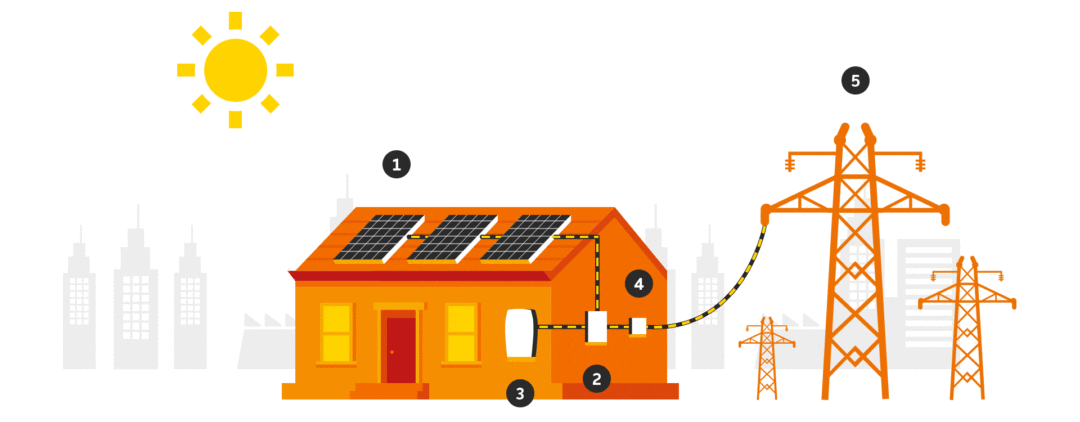
\includegraphics[scale=0.4]{figures/References/NetMetering.PNG}
    \\Image from \cite{Encorsolar}
    \caption{How Net Metering Works}
    \label{fig:NetMetering}
\end{figure}

\section{Types Of Losses}
\label{section:sec01_02} 

Electricity access plays an important role in the development of the society. The population grows in hunger for more power to supply their needs, posing more and more challenges for the energy sector. One of the key factors that affect the efficiency of power distribution is system loss, which refers to the energy that is not received by the consumer. As illustrated in Figure \ref{fig:Losses}, there are two types of losses: technical and non-technical losses. Technical loss is inherent due to the physical delivery of electricity through distribution lines and other substation equipment. These are usually taken into account and are foreseen by the distributors. Non-technical losses (NTL) are results of unidentified energy flows, usually from illegal connection, tampering of meters and erroneous reading \cite{Glauner}.

\begin{figure} [H]
    \centering
    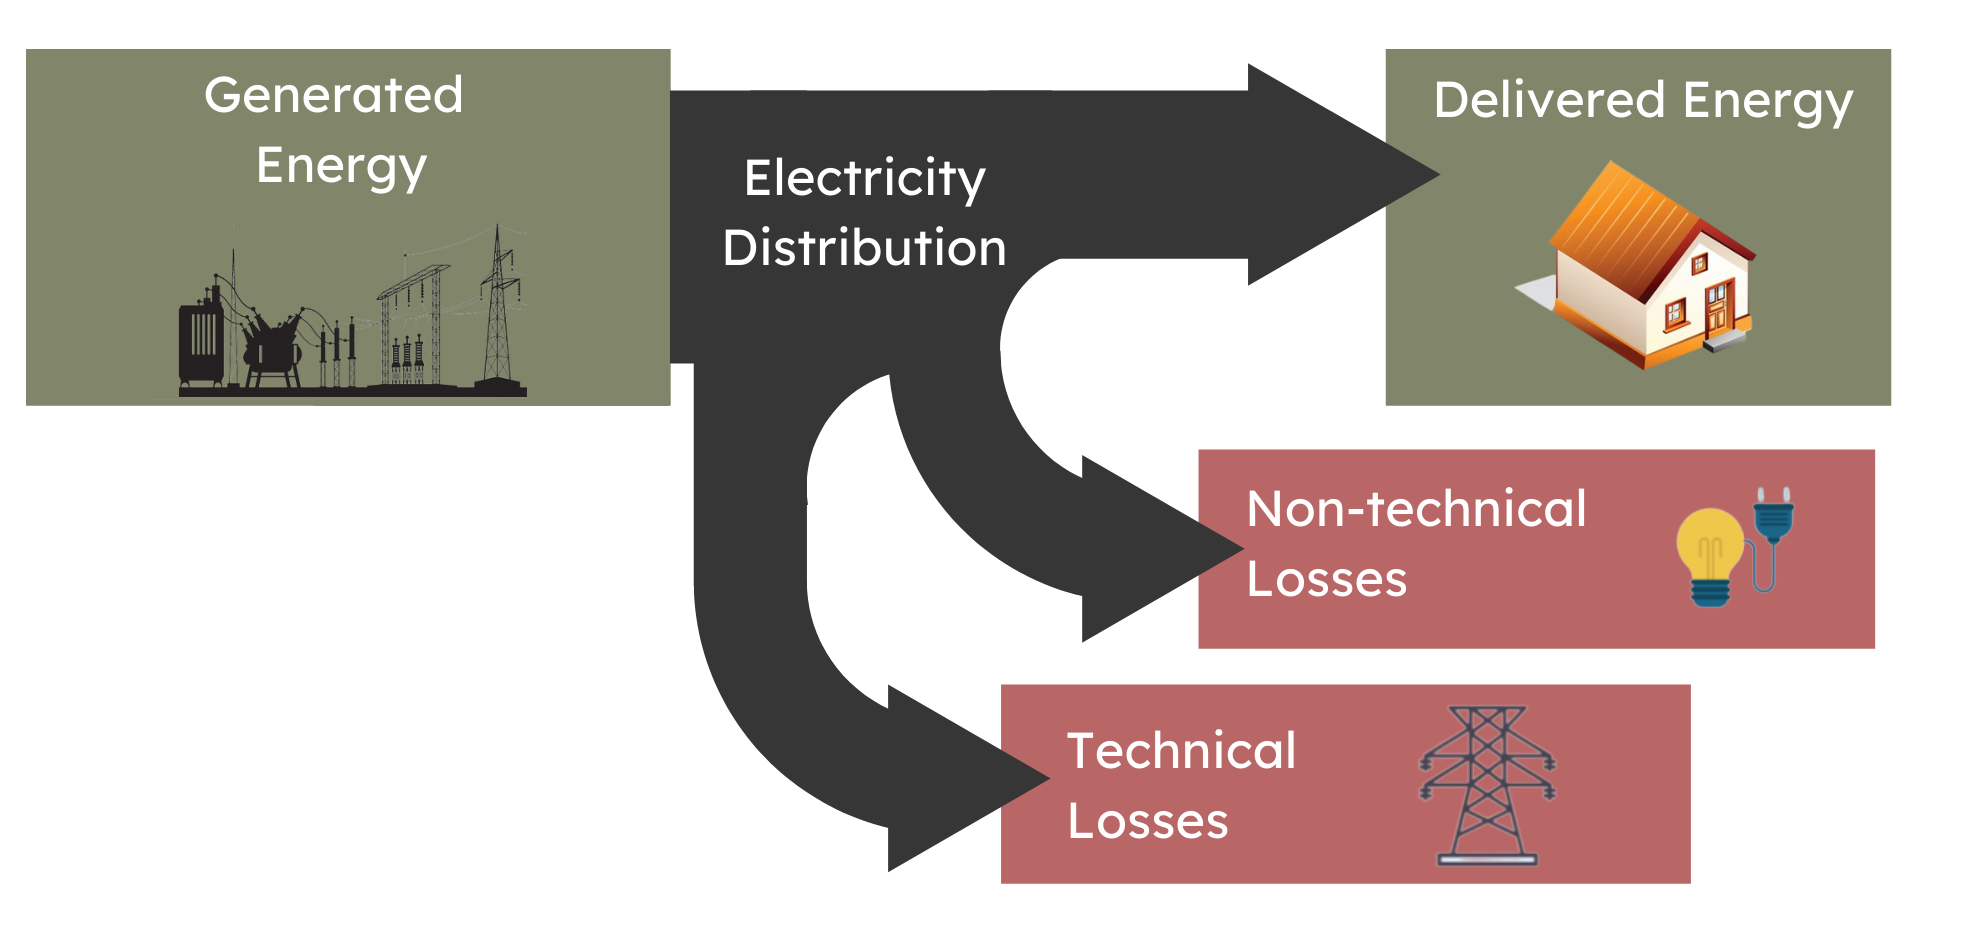
\includegraphics[scale=0.3]{figures/References/Losses.PNG}
    \caption{System Loss}
    \label{fig:Losses}
\end{figure}

\section{Electricity Theft}
\label{section:sec01_03} 

 Electricity theft is caused by pilferers that perform illegal alterations on the system in order to reduce their own power consumption reading. In some cases, it results to an increase in the electricity consumption recorded by the smart meter of other users \cite{Tao}. Non-technical loss in smart grids that are mostly due to energy theft, has become a major enduring challenge in the power distribution industry worldwide \cite{Kim}. For the electricity providers, electricity theft is a big nuisance and they have been trying to detect such activities by deploying smart meters (SMs) to modernize current power grids and energy metering functions. However, these SMs are very vulnerable to various types of attacks and may make energy theft easier to commit \cite{Kim}. For the consumer, a discrepancy in meter reading might mean paying for more than electricity consumed.

%\section{Electricity Theft Detection and Identification}
%\label{section:sec01_04} 

 Due to the nature of non-technical loss during transmission of electrical energy, it is difficult for the utility companies to detect and apprehend the people responsible for theft. Various works claim that energy theft in advanced metering infrastructure (AMI) is becoming more prevalent \cite{Jiang}. With this, the energy sector is challenged to call for the development of effective theft detection techniques. 
 
 \section{Project Flow and Organization}
\label{section:sec01_05} 

    Chapter 2 discusses the related works about system loss reduction, electricity theft, and some detection electricity theft methods. A section will also be given to understanding related works on rooftop photovoltaics in theft detection.
    
    Chapter 3 includes the statement of the problem that lead to the idea of the project and the objectives together with its scope and limitations.
    
    Chapter 4 contains the methodology explaining how the project is implemented. It consists of the overview, modelling of the test system, implementation of theft detection algorithms, and the performance metrics calculation.
    
    Chapter 5 compares the results and discusses how PV and Net Metering affects the different algorithms used.
    
    Chapter 6 contains the conclusion and recommendation that the proponents have for this project.

\cleardoublepage{}

%%%%%%%%%%%%%%%%%%%%%%%%%%%%%%%%%%%%%%%%%%%%%%%%%%%%%%%%%%%%%%%%%
\chapter{Background and Related Work\label{cha:chap02}}
	
	In this chapter, different types of electricity theft as well as works related to electricity theft detection algorithms are discussed and analyzed. The concept of system loss is also expanded in this chapter as well as the current state of electricity theft detection algorithms with regards to systems with rooftop photovoltaics.
	
\section{System Loss Reduction}
\label{section:sec02_01}

System loss is present in all electrical systems. Electrical equipment and materials, such as transmission lines and transformers that are used in distribution infrastructures, dissipate heat and energy is wasted in the process. Figure \ref{fig:ShortLine} shows a model for a short transmission line. Transmission lines are classified according to their lengths; with the short line as the most basic model. When power is transmitted along the line, a difference in power is caused by the series impedance of the line. The power loss is denoted as \(P_{losses} = I_s^2(R+j\omega L)\) \cite{Benedict}.

\begin{figure} [H]
    \centering
    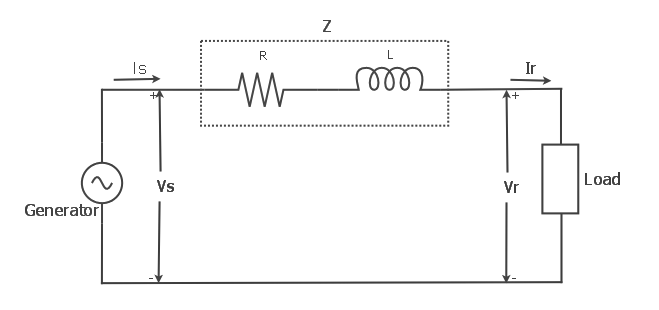
\includegraphics[scale=0.6]{figures/References/ShortLine.png}
    \caption{Transmission Lines - Short Line Model}
    \label{fig:ShortLine}
\end{figure}

System loss significantly affects the revenue of electric utilities, and even its customers. This motivates growing countries to develop different methods and initiatives to reduce system loss, involving the government and the general public in the process. In the Philippines, the Manila Electric Company (Meralco) implements reduction initiatives that reduce both technical and non-technical losses. \cite{MeralcoProgram} 

For technical loss reduction, re-configuring and upgrading distribution systems are regularly done to improve the overall efficiency of electric power distribution across the country. This includes the installation of capacitor banks and optimizing the loading of distribution transformers. 

For non-technical loss reduction, the Anti-Pilferage Law (Renewable Energy Act of 1998) \cite{AntiPilferageAct} is strictly implemented to apprehend offenders and prevent electricity theft. Despite this, different types of electricity theft are now prevalent, even in advanced electrical systems like AMIs. To combat this, our current theft detection methods will need to adapt.

\section{Electricity Theft}
\label{section:sec02_02}

There are various types or methods of electricity theft. These methods can range from direct hooking from line to cyber-attacks on smart meters. However, physical methods of theft are no longer the only type of attack. With the increasing number of smart meters, cyber-attacks are on the rise \cite{TPSrivera}\cite{Velasco}. Electricity theft could be divided into three groups, namely, interruption of measurement, tampering of stored demand, and network hijacking as follows \cite{Jiang}:

\begin{enumerate}
	\item Interruption of measurement is done by the attacker by either disconnecting the meter or via meter inversion. This takes place before the meter could make a record of the consumed electricity.
    \item Tampering of stored demand occurs when the attacker accesses the administrative interfaces with passwords and erases the stored value of the measured electricity consumption.
    \item Network hijacking is completed when the attacker is able to intercept communication and inject traffic to the smart meter allowing a delivery of forged data to the smart meter.
\end{enumerate}

Clients of electric companies make attempts at stealing energy provided by their very own electric companies, with varying degrees of success. The most common reason for this phenomenon is the attempt to save money. Among the many known methods of theft, the most popular ones are: making a concealed connection and a mechanical blockade of the analog mechanism.  Energy theft by tampering with a digital smart meter is much more difficult and requires specialized knowledge, which greatly narrows the circle of clients whose specialized knowledge enables them to perform unauthorized manipulation of the meter \cite{Kosek}. 

\section{Electricity Theft Detection Methods}
\label{section:sec02_03}

Electricity theft detection methods aim to distinguish pilferers in an electrical system. Theft detection methods that are used in smart grids include the use of a check meter. A check meter is installed upstream as basis, which compares its reading to the sum of individual smart meter readings of downstream households. The check meter's role is to check whether or not there is a mismatch between the total reading and the individual household readings. 

To illustrate how theft detection works, an example of a smart grid is shown in Figure \ref{fig:SmartGridM3}. In this case, \(M3\) commits a cyber-attack which manipulates their own smart meter reading from 40 kWh to 20 kWh. However, this does not affect the reading of the check meter; instead, the check meter still reads 40 kWh for \(M3\) as shown in Equation \ref{equation:CMEquation}. 

\begin{figure} [H]
    \centering
    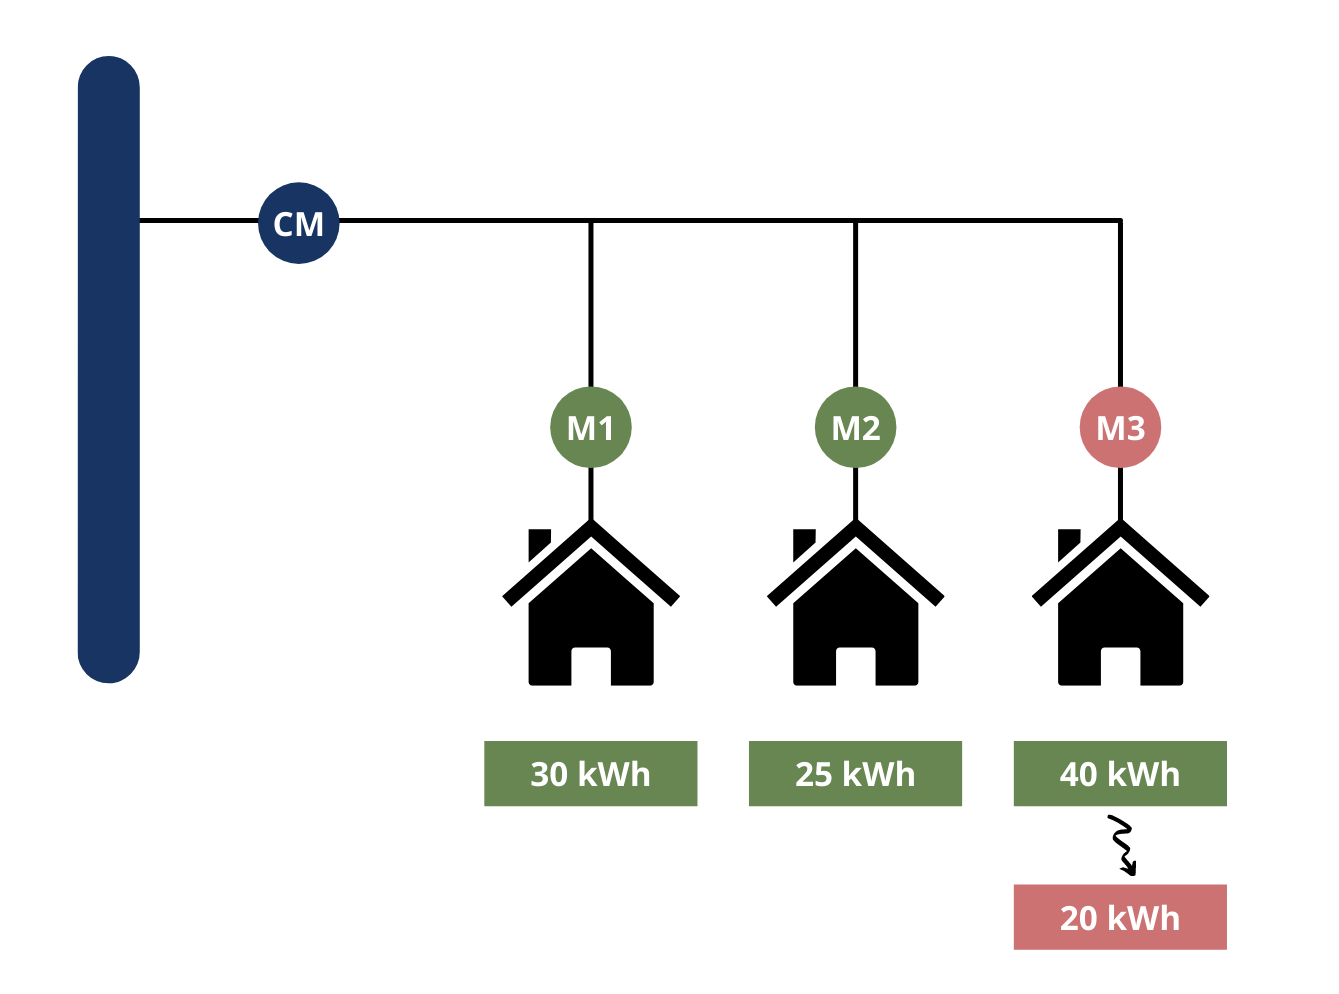
\includegraphics[scale=0.35]{figures/References/SmartGridM3.png}
    \caption{Smart Grid Model - M3 as Pilferer}
    \label{fig:SmartGridM3}
\end{figure}

\begin{equation} \label{equation:CMEquation}
\begin{split}
& CM = {M1 + M2 + M3 + P_{techlosses}} \\
& CM = {30 kWh + 25 kWh + 40 kWh + P_{techlosses}} \\
& CM = 95 kWh + P_{techlosses}
\end{split}
\end{equation}

The manipulated value of \(M3\) is taken into account when calculating for the sum of the individual smart meter readings in the grid. As seen in Equation \ref{equation:IndivMeters}, the sum of the individual readings is not equal to the check meter reading which is 95 kWh. The obvious mismatch means that there is pilferage in the system.

\begin{equation} \label{equation:IndivMeters}
\begin{split}
& SUM(M1,M2,M3) = 30 kWh + 25 kWh + 20 kWh \\
& SUM(M1,M2,M3) = 75 kWh
\end{split}
\end{equation}

However, it is important to note that \(P_{techlosses}\) is also relevant in the equation. In real life situations, \(P_{techlosses}\) is not equal to zero. Therefore, even if there is no pilferage in the system, there would still be a mismatch between the check meter reading and the sum of all individual meter readings. This complicates electricity theft detection especially in large systems. 

Electricity theft detection methods have also evolved to adopt several machine learning techniques and use it to detect pilferage in a system. A research by \cite{Nagi} used Support Vector Machines (SVM) to preselect suspicious customers using historical customer consumption data. The suspected customers are then visited on-site for inspections. In this method, historical data must be collected and used to train and test the SVM model. SVM classifiers are used for binary classification problems using data with either linear or non-linear relationships. Labelled training data from two classes are mapped as points in space and a separating hyperplane is solved to separate the two classes with maximum margin. Testing data is then mapped into the same space and outputs a predicted class based on the same hyperplane \cite{Hsu}.

Theft detection methods based on artificial neural networks (ANN) are also quickly becoming popular \cite{Messinis}. In a study by \cite{Zheng}, a wide and deep convolution neural network (CNN) model is proposed as a model for theft detection in smart grids. The resulting model was able to outperform other theft detection methods such as SVM. The idea of ANN is inspired by the biological model of a neuron. A typical neural network consists of an input layer, an output layer, and several hidden layers in between \cite{Larochelle}. Each layer is made up of multiple neurons that use the neurons of the preceding layer as its inputs and passes its output to the succeeding layer \cite{Bengio}. Like SVM, ANNs are trained with labelled data and is evaluated using new, unseen data.

Reference \cite{MendiolaPedrasa} proposed a method on anomaly coefficient calculation to be used as linear equations to detect pilferage. This method has been demonstrated to detect a single pilferer in a low-voltage network with household smart meters and a check meter. His succeeding works improved on this algorithm as it can now be used to detect multiple pilferers and work with small percentages of system losses. The algorithm was later tested on a larger test system with 60 households in a low-voltage network and varying theft behavior. The lowest accuracy rate was 89\% and the lowest average accuracy was 97\%. The highest accuracy and highest average accuracy are both 100\% \cite{MeralcoProgram}.

The algorithms that were stated above were developed and tested on systems that do not have rooftop PVs and Net Metering. The following section will discuss the technicalities and the current state of electricity theft detection in systems with PV and Net Metering. 

\section{Electricity Theft Detection in Systems with PV and Net Metering}
\label{section:sec02_04}

Increasing levels of rooftop PV penetration (defined as the ratio of the total number of households with PV installation to the total number of households) introduces technical challenges that can affect the distribution grid. Related works show that factors such as voltage and current imbalance, and power losses received the most attention in recent publications \cite{Alboaouh}. As discussed in \ref{section:sec01_01}, net metering allows excess energy produced by rooftop PVs to flow back to the grid. This can also cause complications to the distribution grid because net metering introduces the concept of 'negative' power flow in the system.

As the aforementioned complexities are added to electrical systems with PV and Net Metering, current electricity theft detection methods may also be affected. To further explain this, it is important to know how theft detection algorithms work when subject to different penetration levels of PV and Net Metering. Different cases wherein pilferers manipulate their own PV generation also pose a threat to power distribution companies. 

Reference \cite{Yuan} presented an algorithm which uses the least squares approach to detect electricity theft. Their research focused mainly on cases where pilferers increase the value of their PV generation meter reading for extra profit. Their algorithm was tested on electrical systems that use individual meters for PV generation, and check meters to detect electricity theft. Their research did not mention the use of Net Metering.

Reference \cite{Ismail} adopted deep machine learning techniques to detect electricity theft cyber-attacks in a PV system. Their research also developed their own dataset, including different cyber-attack functions, to realistically simulate theft. Different deep machine learning models were tested, and their metric scores were compared with each other. However, the effect of PV and Net Metering wasnot highlighted and quantitized; they focused on testing their machine learning models on datasets with PV.

\section{Background Summary}
\label{section:sec02_05}
The research done by \cite{Nagi} and \cite{Zheng} in using machine learning techniques for detecting electricity theft showed outstanding results. However, there are no PVs in the electrical systems they used. On the other hand, both works by \cite{Yuan} and \cite{Ismail} explored theft detection algorithms on test networks with PV installation. However, the focus was on the performance of the algorithms themselves and not the effect of PV and Net Metering on electricity theft detection. Therefore, there is a need to characterize the effect of PV and Net Metering on the performance of electricity theft detection to bridge the gap in knowledge.

\cleardoublepage{}

%%%%%%%%%%%%%%%%%%%%%%%%%%%%%%%%%%%%%%%%%%%%%%%%%%%%%%%%%%%%%%%%%%
\chapter{Problem Statement and Objectives \label{cha:chap03}}

\section{Problem Statement}
\label{section:sec03_01}

The use of rooftop photovoltaics and Net Metering are on the rise. However, there have only been few discussions on the effects of such technologies with our current types of electricity theft detection algorithms. This becomes problematic when a system heavily relies on current algorithms that may not be able to detect pilferers accurately.

\section{Objectives of the Project}
\label{section:sec03_02}

This project aims to analyze the effect of rooftop photovoltaics and Net Metering on the performance of different electricity theft detection algorithms. The algorithms were tested on different datasets with varying presence of PV and Net Metering. Their accuracy, precision, recall, and F1 score was calculated and discussed.

\section{Scope and Limitations}
\label{section:sec03_03}

This project will test three theft detection algorithms: Support Vector Machine (SVM), and Artificial Neural Network (ANN), and Anomaly Coefficient Calculation. The performance of each algorithm will be tested on different datasets, each with varying presence of PV and Net Metering. The simulation will be limited to the detection of electricity theft through a cyber-attack, where the pilferer manipulates their own smart meter reading.

\cleardoublepage{}

%%%%%%%%%%%%%%%%%%%%%%%%%%%%%%%%%%%%%%%%%%%%%%%%%%%%%%%%%%%%%%%%%
\chapter{Methodology\label{cha:chap04}}

\section{Overview}
\label{section:sec04_01}

This chapter discusses the methodology of the project. Each section provides a comprehensive explanation of each step, from the modelling of test systems up to the implementation of theft detection algorithms. 

Selected household load and PV generation data were extracted and were used as inputs to a test network model. The power-flow of the network was performed to simulate meter readings across different PV and Net Metering scenarios. Table \ref{tab:Dataset} shows the seven dataset categories, with each of them having different PV and Net Metering penetration levels. 

\begin{table}[]
\centering
\begin{tabular}{|c|c|c|}
\hline
\multicolumn{1}{|c|}{\textbf{Dataset}} & \multicolumn{1}{c|}{\textbf{PV Penetration \%}} & \multicolumn{1}{c|}{\textbf{NM Penetration \%}} \\ \hline
D1                             & 0                         & 0                         \\ \hline
D2                             & 20                        & 0                         \\ \hline
D3                             & 70                        & 0                         \\ \hline
D4                             & 20                        & 20                        \\ \hline
D5                             & 20                        & 70                        \\ \hline
D6                             & 70                        & 20                        \\ \hline
D7                             & 70                        & 70                        \\ \hline
\end{tabular}
\caption{\label{tab:Dataset}Dataset Categories}
\end{table}

Electricity theft in the form of smart meter manipulation was applied on the simulated data. The desired features were extracted, and the datasets were labeled. 

Finally, these datasets were used as inputs to three different theft detection algorithms: Support Vector Machine (SVM), and Artificial Neural Network (ANN), and Anomaly Coefficient Calculation. The performance metrics of each algorithm were then calculated and assessed.

\section{Modelling of Test Systems}
\label{section:sec04_02}

\subsection{Household Data Preparation}
\label{section:sec04_02_01}

An Australian distribution network with household load and rooftop PV generation data was used as the primary sample data \cite{AUResidential}. It was made available by Ausgrid, an electric utility in Sydney and nearby areas in New South Wales. The dataset contains meter readings from 300 customers taken at half-hourly intervals, and with the following parameters: PV production, generator capacity, electricity consumption, and off-peak-controlled consumption. The postcode location map and the irradiation map are shown in Figure \ref{fig:AusgridMaps}. Irradiance is defined as the radiant energy per unit time that strikes a unit horizontal area per unit wavelength interval \cite{Abraham}. By observing the map, it can be inferred that the irradiation data of the households in the area covered by Ausgrid are closely correlated to each other. The data was collected from \cite{AUData}.

\begin{figure} [H]
    \centering
    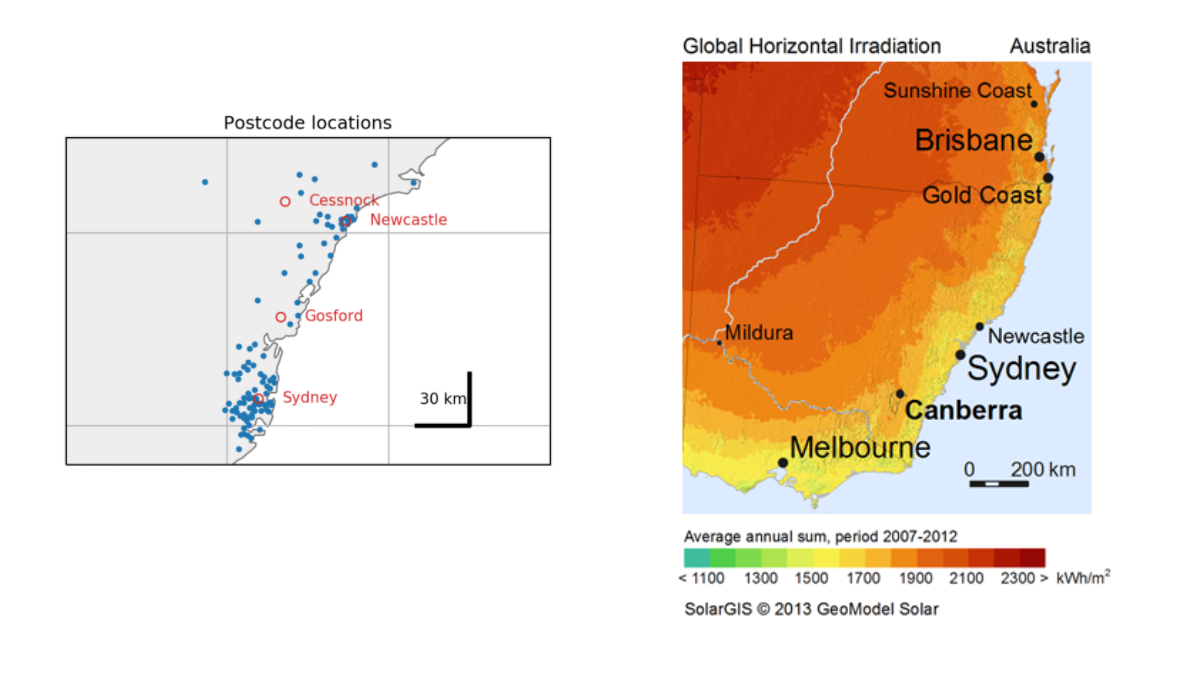
\includegraphics[scale=0.5]{figures/References/PostcodeLoc_Irradiation.png}
    \\Image from \cite{AUData}
    \caption{Ausgrid Data Location and Irradiation Maps}
    \label{fig:AusgridMaps}
\end{figure}

Data cleaning is necessary to maintain consistency all throughout the process. The following requirements and steps were followed in preparing the household load dataset. Python was used in this process.

\begin{enumerate}
	\item Only households with complete general consumption and gross generation data in the selected dates were selected. This reduced the number of customers of the Ausgrid data from 300 to 161.
    \item One week worth of data was extracted. The week of December 5-11, 2010 was chosen for its similar temperature compared to the summer season in the Philippines.
    \item The general consumption data and the gross generation data were collected and converted into individual customer profiles to be used as input load curves and PV generation curves respectively. Other irrelevant parameters, like the controlled load consumption data, were not included.
\end{enumerate}

After the data cleaning process, the data is now ready to be used as input to the test network. The following section dissects the network modelling process and its specifications.

\subsection{Network Modelling}
\label{section:sec04_02_02} 

\subsubsection{Low-Voltage Test Feeder}
\label{section:sec04_02_02_01} 

The network was modeled after the IEEE European Low Voltage Test Feeder. It was designed by the Test Feeders Working Group of the Distribution System Analysis Subcommittee of the Power Systems Analysis, Computing, and Economics (PSACE) Committee \cite{PESFeeder}. The feeder is at the voltage level of 416 V (phase-to-phase). Its base frequency of 50 Hz was kept at the same level. The other parameters such as the line and substation codes were kept at a default setting. 

There are 55 PQ loads that are connected to the main substation. Additionally, we placed check meters to group the households according to their locations. The topology of the system is shown in Figure \ref{fig:SystemTopology}. The area under each check meter is also highlighted in red. The following subsections will expound on how the household loads were modeled, depending on the presence of PV and Net Metering. 

\begin{figure} [H]
    \centering
    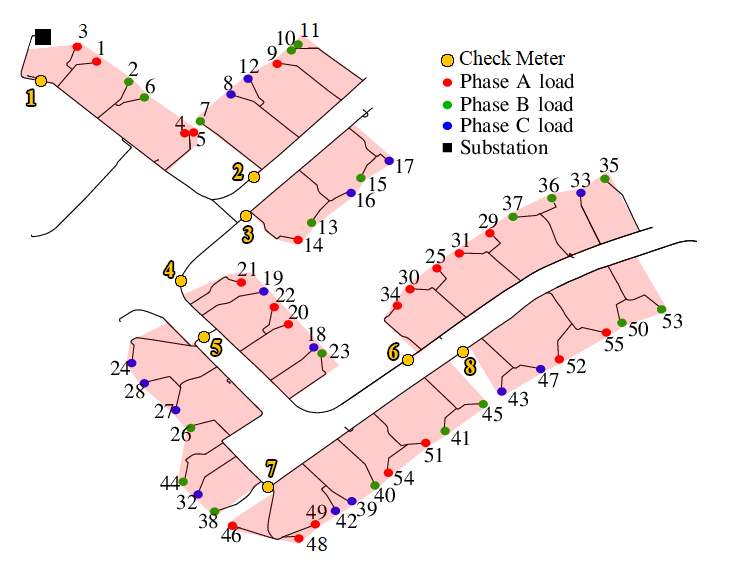
\includegraphics[scale=0.7]{figures/References/CheckMeter198.png}
    \\Image from \cite{PESFeeder}
    \caption{System Topology}
    \label{fig:SystemTopology}
\end{figure}

\subsubsection{Household Loads}
\label{section:sec04_02_02_02} 

Each household was modelled as a PQ load, the load curve of each household was derived from the Ausgrid data. Additionally, smart meters were connected to every household to measure the power reading or consumption of each load. The sample load curve in \ref{fig:LoadCurve} shows the kWh power reading of a household in 1 week at a half-hour interval.

\begin{figure} [H]
    \centering
    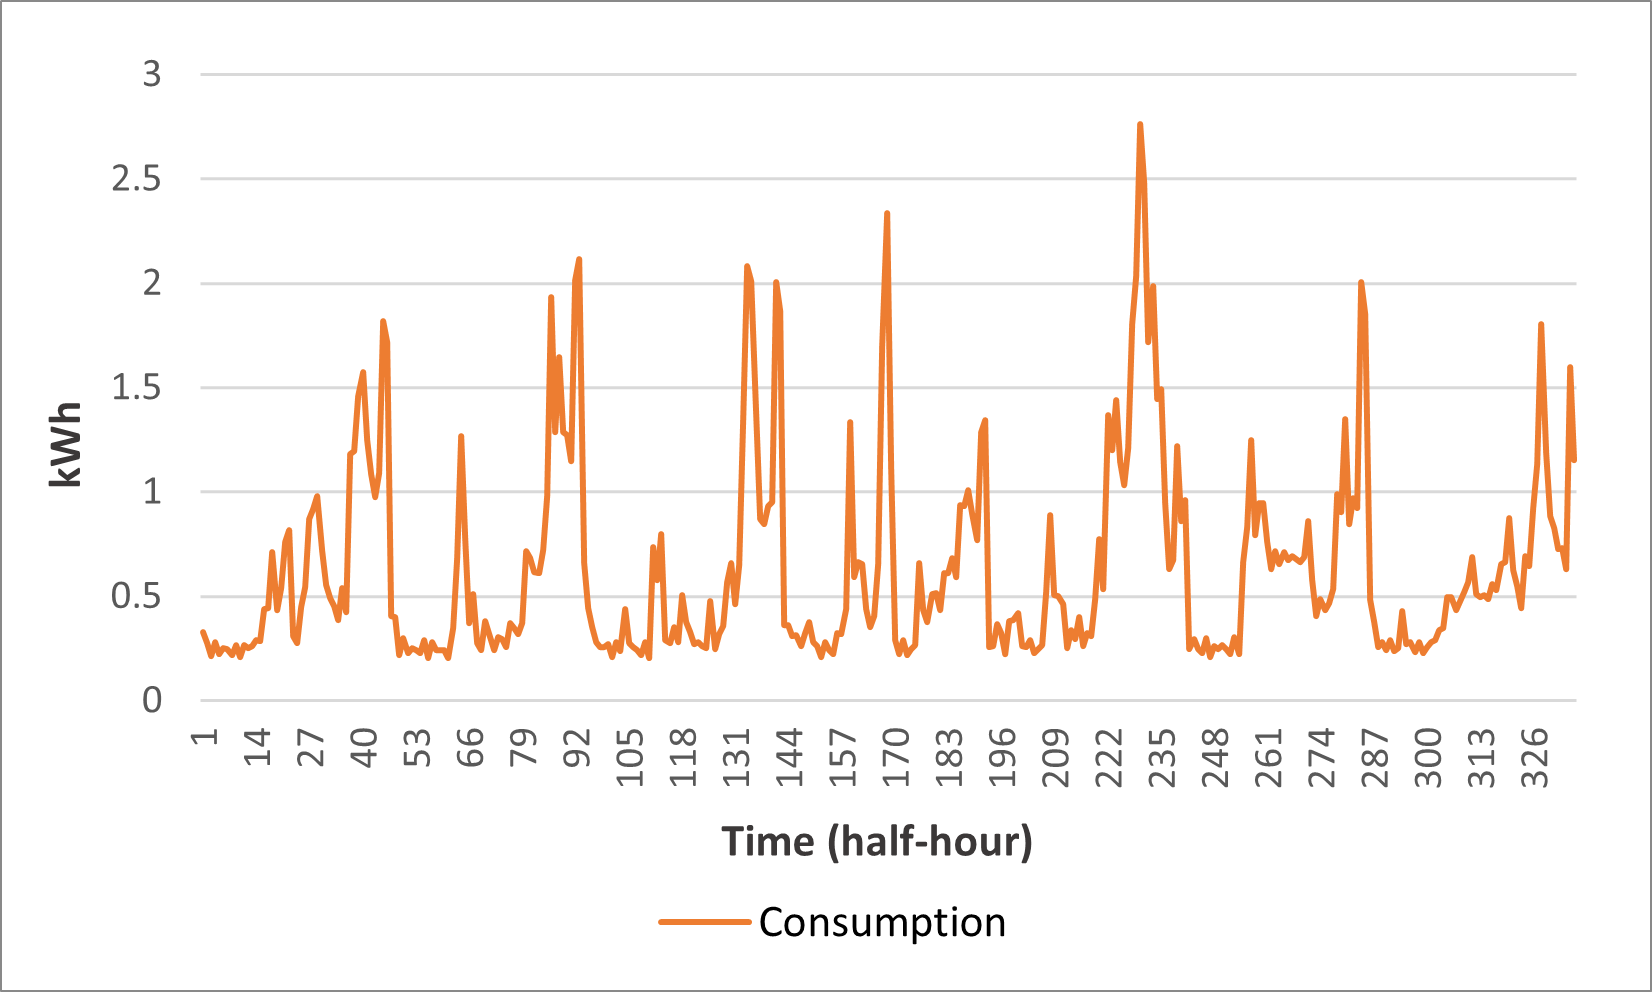
\includegraphics[scale=0.7]{figures/References/load_curve.png}
    \caption{Household Load Curve - 1 Week }
    \label{fig:LoadCurve}
\end{figure}

\subsubsection{Rooftop PV and Net Metering Model}
\label{section:sec04_02_02_03} 

To simulate a household with a rooftop PV, an additional generator object was connected to the PQ load. The PV generation data from Ausgrid is used as an input for the generator. The household with a rooftop PV would have two curves: a load curve that represents its consumption, and a generation curve that represents its PV generation. For a household with Net Metering, excess energy produced by the rooftop PV will be exported to the grid. The exported energy to the grid by household \(i\) is given by
\[P_{excess, i}= P_{generation, i} - P_{consumption, i}\]

The graph in Figure \ref{fig:LoadandGenCurve} shows the kWh power reading of a household with Net Metering, together with its PV generation in 1 week at a half-hour interval. Excess energy is exported during the time-frames where PV generation is greater than the household's consumption.

\begin{figure} [H]
    \centering
    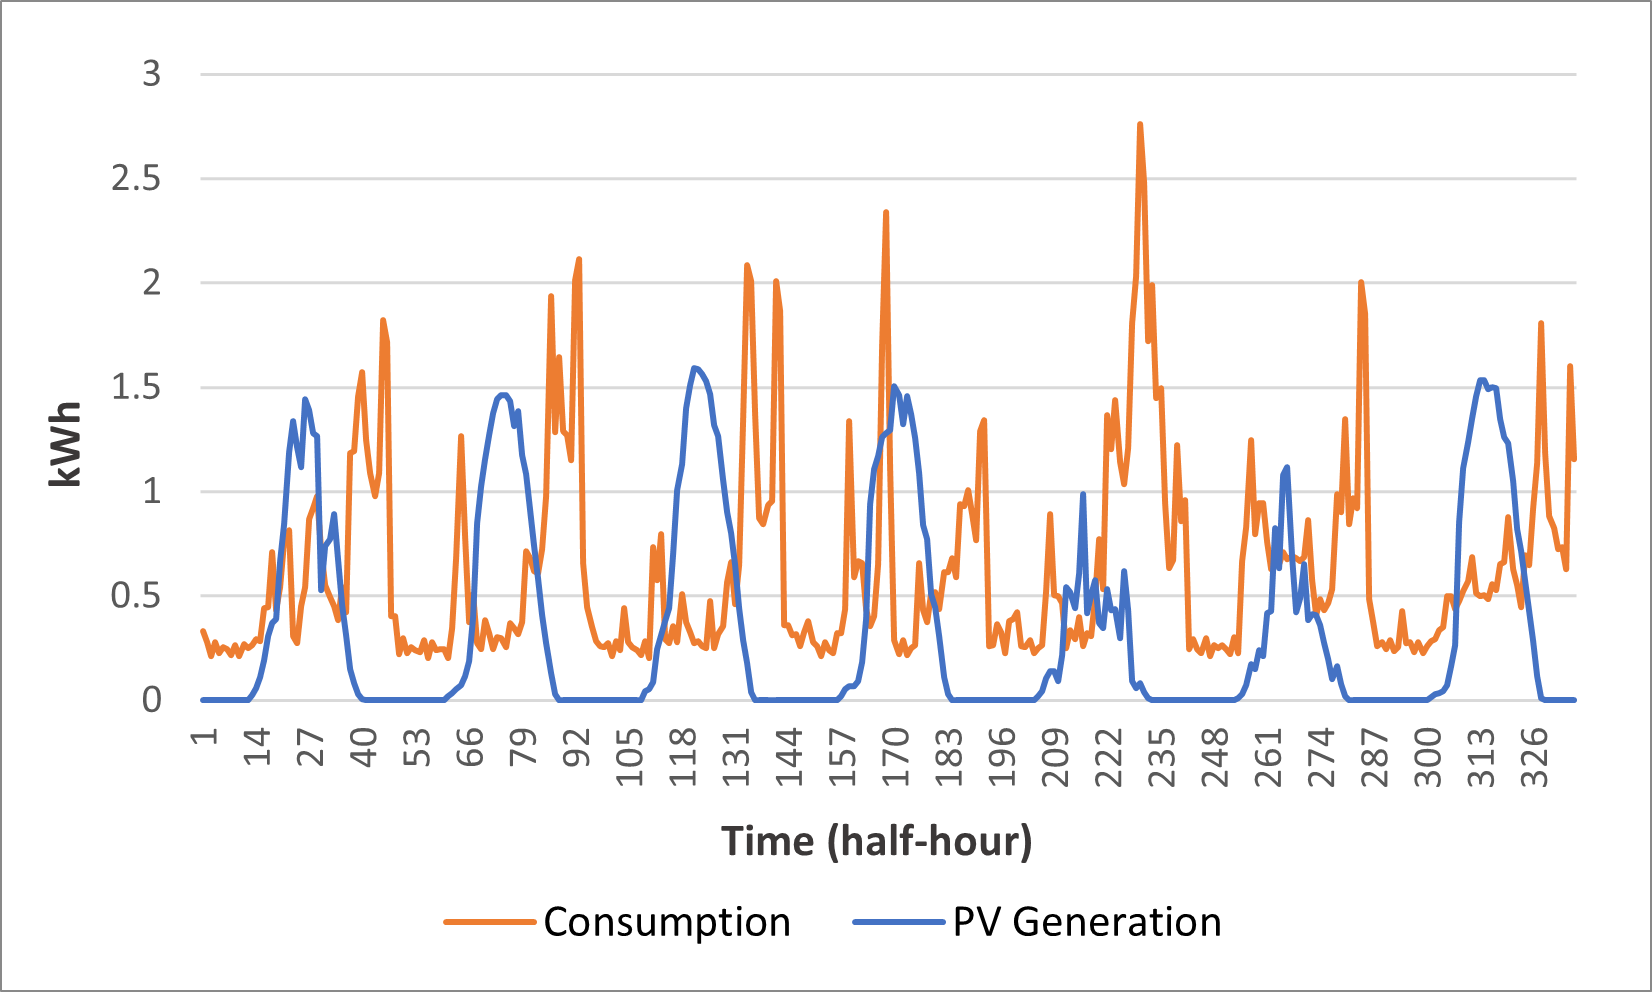
\includegraphics[scale=0.7]{figures/References/pv_nm_chart.png}
    \caption{Household with PV and NM - Load and Generation Curve - 1 Week}
    \label{fig:LoadandGenCurve}
\end{figure}

For a household with PV but no Net Metering, excess energy is not exported back to the grid. To model this behavior, the PV generation curve was altered such that PV generation is clipped to the household consumption curve. This way, all the energy produced from the rooftop PV is consumed by the household. Figure \ref{fig:LoadandGenCurve_noNM} shows the counterpart of Figure \ref{fig:LoadandGenCurve} if the household has no Net Metering.

\begin{figure} [H]
    \centering
    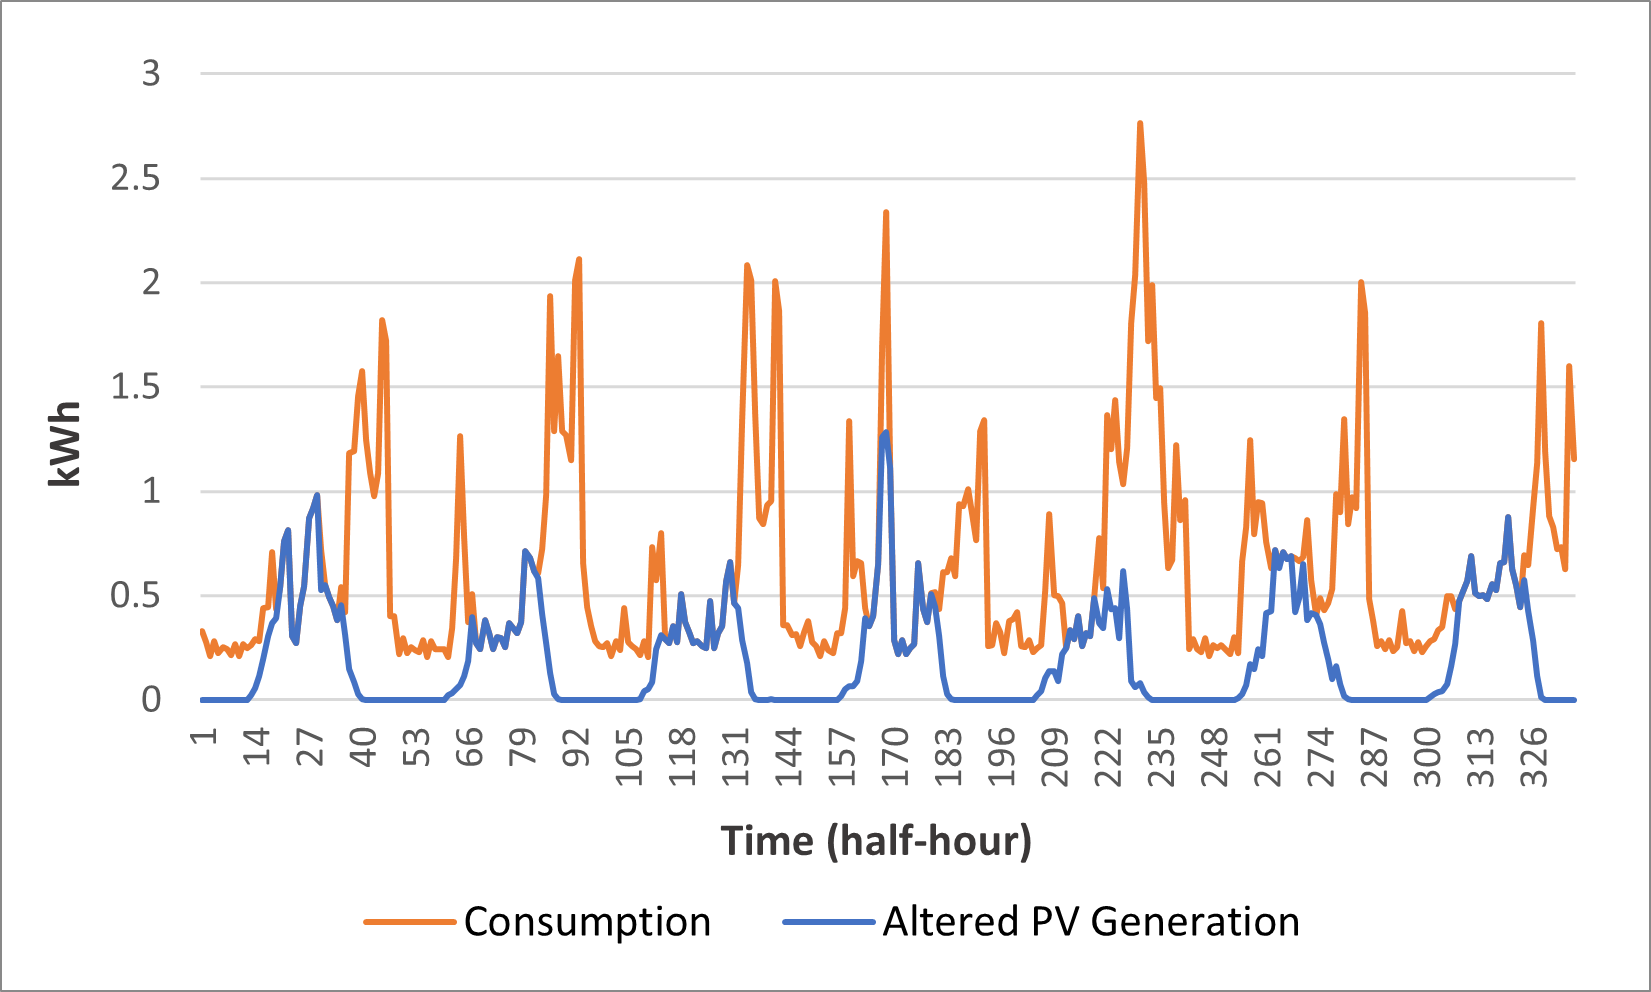
\includegraphics[scale=0.7]{figures/References/pv_wo_nm_chart.png}
    \caption{Household with PV only - Load and Generation Curve - 1 Week}
    \label{fig:LoadandGenCurve_noNM}
\end{figure}

After modelling the test network, it is now ready for simulation. The next section discusses the details of the power-flow simulation, and what outputs were exported from the simulations.

\subsection{Power-flow Simulation}
\label{section:sec04_02_03} 

After modelling the test network, OpenDSS was used for power-flow simulation. It is a comprehensive power system simulation software that allows users to run power-flow calculations on a system. The specifications of the feeder that were discussed in are required to run the power-flow simulation. Additionally, the duration of the simulation would also need to be specified. In this project specifically, OpenDSS was used to export the time-series data from the check meters and the individual household meters after the simulation. 

As seen in Figure \ref{fig:SystemTopology}, there are 55 households that are connected to the substation, and 8 check meters were assigned based on the geographical locations of the households. To highlight the effect of Net Metering and rooftop PVs on electricity theft detection, the penetration levels of PV and Net Metering were varied. The PV penetration levels were varied between high (70\% of the households have PVs), low (20\% of the households have PVs) and zero (0\% of the households have PVs). For the cases with PV penetration, the Net Metering penetration levels were also varied between high, low, and zero. This resulted in seven different combinations, or seven dataset categories as seen in Table \ref{tab:Dataset}.

For example, at 70\% PV and 20\% Net Metering, the number of households with PV is \(\lfloor55\times0.7\rfloor=38\) and the number of households with both PV and Net Metering is \(\lfloor38\times0.2\rfloor=7\). Net Metering can only be installed on households with rooftop PV.

For each of the seven datasets, 110 week-long simulations were done to serve as benign data or data without theft. Subsequently, the power readings of the check meters and household meters were exported. The reasoning behind the number of simulations is explained in Section \ref{section:sec04_02_04}.

\subsection{Electricity Theft Representation}
\label{section:sec04_02_04}

After the power-flow simulation, each week-long simulation was replicated to add electricity theft. The theft was represented as a cyber-attack, where the pilferer manipulates their own smart meter reading. For each week-long simulation, only one household was chosen to be a pilferer.

The theft was represented as a multiplier \(k_{et}\) to a household's meter reading. \(k_{et}\) was randomly generated using a Gaussian Distribution curve with a mean of 0.5 and standard deviation of 0.05. The minimum and maximum values of \(k_{et}\) are 0.35 and 0.65 respectively; both values are 3 standard deviations away from the mean. \(k_{et}\) is unique for every week-long simulation from Section \ref{section:sec04_02_03}.

The theft duration or frequency was varied to be either continuous or half-day; these two were classified as frequency A and frequency B respectively. Frequency A will be manipulating the household meter reading for one whole day and frequency B will only do this for half of the day, from 6AM to 6PM. This was done to add character to the pilferer since in real time pilferers usually steal electricity at their peak usage time.

With each of the 55 households simulated to be a pilferer, and with two varying frequencies of theft, the resulting data consists of \(55\times2=110\) week-long simulations for each of the seven dataset categories. The resulting data represents the malicious data. 

\subsection{Features and Labelling}
\label{section:sec04_02_05}
Dataset features determine the properties that describe the data points of a dataset. In the context of electricity theft detection, these features are usually customer time-series data derived from active energy consumption curves \cite{Messinis}. The following subsections will discuss the features for SVM, ANN, and Anomaly Coefficient Calculation. The difference between the features for SVM and ANN, and the features of Anomaly Coefficient Calculation will also be discussed.

\subsubsection{Features for SVM and ANN}
\label{section:sec04_02_05_01}
For theft detection algorithms SVM and ANN, the chosen features are the meter readings of each household and the \% loss error of each check meter. Check meter readings are essentially the total power consumption of all downstream households, together with technical losses from the transmission lines. Table \ref{tab:CheckmeterMem} shows which households are under each check meter, as derived from Figure \ref{fig:SystemTopology}. These check meters are usually out of reach from the public and thus, are rarely manipulated.

\begin{table}[H]
\centering
\begin{tabular}{|
>{\columncolor[HTML]{FFFFFF}}c |
>{\columncolor[HTML]{FFFFFF}}c |}
\hline
{\color[HTML]{333333} \textbf {Check Meter}} & \textbf {Households}     \\ \hline
1                                  & 1, 2, 3, 4, 5, 6                   \\ \hline
2                                  & 7, 8, 9, 10, 11, 12                \\ \hline
3                                  & 13, 14, 15, 16, 17                 \\ \hline
4                                  & 18, 19, 20, 21, 22, 23             \\ \hline
5                                  & 24, 26, 27, 28, 32, 38, 44         \\ \hline
6                                  & 25, 29, 30, 31, 33, 34, 35, 36, 37 \\ \hline
7                                  & 39, 40, 41, 42, 45, 46, 48, 49, 51 \\ \hline
8                                  & 43, 47, 50, 52, 53, 55             \\ \hline
\end{tabular}
\caption{\label{tab:CheckmeterMem}Check Meters and Respective Downstream Households}
\end{table}

In a benign dataset, the check meter readings are almost exactly the same as the sum of the individual household meter readings; the small difference accounts for the technical losses from the transmission lines. On the other hand, in a malicious dataset where a pilferer manipulated their meter readings, the difference between the check meter readings and the sum of the household meter readings can be significantly larger. The \% loss error for a check meter \emph{i} was calculated using

\begin{equation}
\label{equation:percent_error}
\% error_i = \frac{\abs{\sum_{n=1}^{k}M_n-CM_i}}{CM_i}
\end{equation}
where \(CM_i\) is the reading of check meter \emph{i} and \(\sum_{n=1}^{k}M_n\) is the sum of the household meter readings under check meter \emph{i}. Thus, the features of the datasets for ANN and SVM are: the \% loss error of the 8 check meters, and the meter readings of the 55 households; this totals to 63 features. 

Every data point in each dataset category are the daily average values of the calculated \% loss error and the week-long meter readings from Section \ref{section:sec04_02_03} and Section \ref{section:sec04_02_04}. At the end of each data point, a label column was added with a value of:
\begin{itemize}
  \item 0, if the data point is benign or there is no theft present
  \item 1, if the data point is malicious or theft is present
\end{itemize}

\subsubsection{Features for Anomaly Coefficient Calculation Method}
\label{section:sec04_02_05_02}

To satisfy the prerequisites of the Anomaly Coefficient Calculation method, the features that were selected differ from the ANN and SVM features. For this method, it was assumed that there is only a single check meter in the network and all households are under it. The altered topology is shown in Figure \ref{fig:SystemTopologyAltered}. Thus, the features for this algorithm are: the check meter readings of Check Meter 1 (main check meter), and the meter readings of the 55 households; this totals to 56 features. 

\begin{figure} [H]
    \centering
    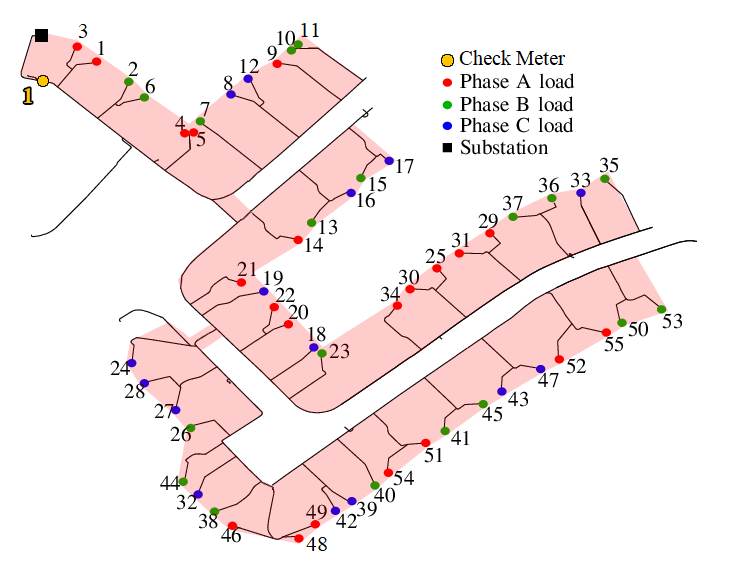
\includegraphics[scale=0.7]{figures/References/CheckMeter198_altered.png}
    \\Image from \cite{PESFeeder}
    \caption{Altered System Topology for Anomaly Coefficient Calculation Method}
    \label{fig:SystemTopologyAltered}
\end{figure}
\subsection{Dataset Summary}
\label{section:sec04_02_06}

A summary of how each dataset is created is summarized below in Figure \ref{fig:C4.2Flow}. For SVM and ANN, the features are the daily average meter readings and the \% loss error of each check meter. There are a total of 63 features for SVM and ANN with one label. Since there are 55 households, 7 days per simulation, 2 theft frequencies, and 2 types of label, benign and malicious, there is a total of \(55\times7\times2\times2=1540\) data points per dataset. 

For Anomaly Coefficient Calculation, the features are presented as the total substation reading and the half-hourly meter readings. There are a total of 56 features and one label. Given that there are 55 households, with 48 half-hourly readings, 7 days per simulation, 2 theft frequencies, and 2 types of label, there is a total of \(55 \times 48 \times 7 \times 2 \times 2 = 73920\) data points per dataset. 

\begin{figure} [H]
    \centering
    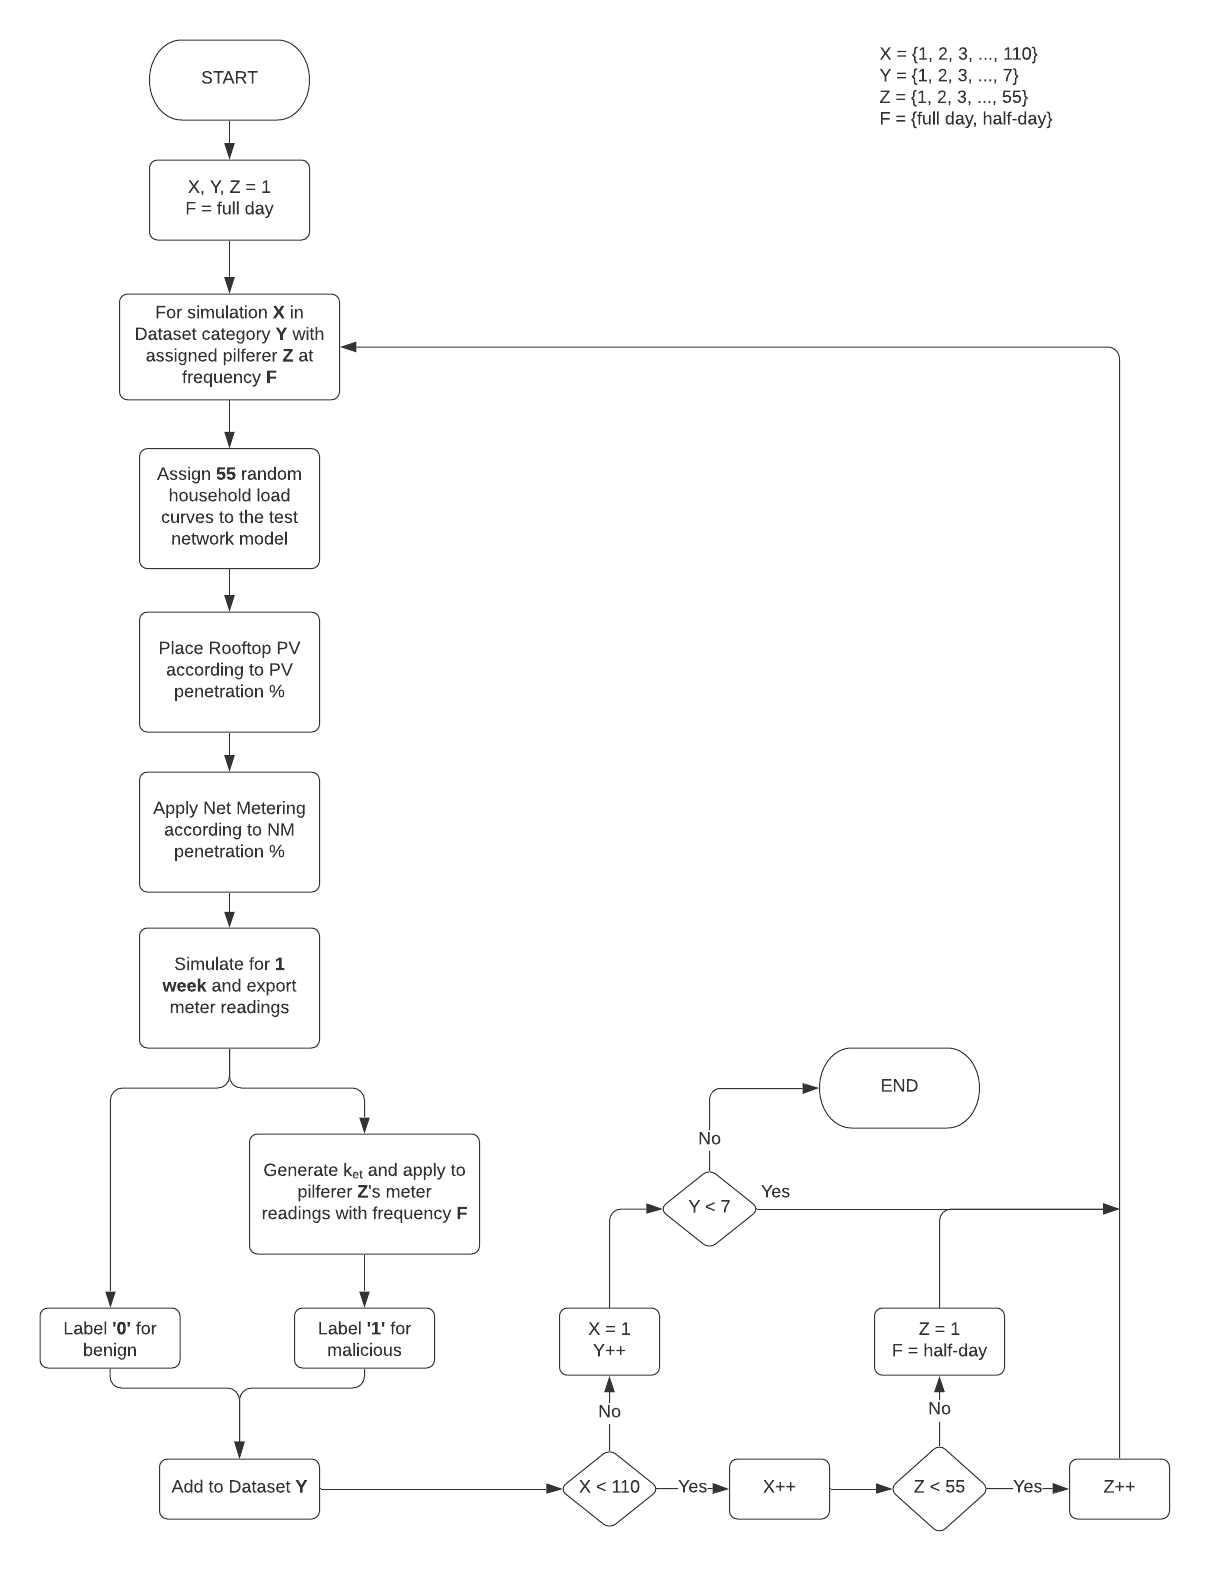
\includegraphics[scale=0.9]{figures/References/C4.2 Flowchart.png}
    \caption{Dataset Creation Procedure}
    \label{fig:C4.2Flow}
\end{figure}

\section{Implementation of Theft Detection Algorithms}
\label{section:sec04_03}

The seven dataset categories created from Section \ref{section:sec04_02} were used and evaluated on each of the three algorithms independently. The SVM classifier was developed using the Scikit-learn library, while the ANN classifier was developed using the Keras library. Both classifiers were written in Python using Jupyter Notebook and were executed using Google Colab Pro virtual machines for fast training and testing times. The third algorithm, Coincident Meter Measurements and Anomaly Coefficient Calculation, was developed using MATLAB.

\subsection{SVM}
\label{section:sec04_03_01} 

An SVM classifier works by solving for a linear hyperplane that separates the classes with maximal margin. Figure \ref{fig:SVM} shows the procedure for SVM from \cite{Hsu}. 

\begin{figure} [H]
    \centering
    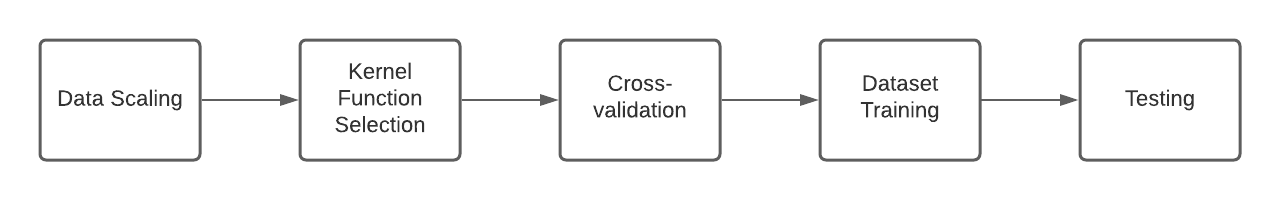
\includegraphics[scale=0.8]{figures/References/SVM.PNG}
    \caption{General Procedure for SVM}
    \label{fig:SVM}
\end{figure}

Initially, the datasets were standardized to a normalized scale such that the data have zero mean and unit variance. This was done to avoid large feature values dominating lower feature values \cite{Hsu}. The datasets were individually standardized using the following formula, where \(X'\) is the standardized value:

\begin{equation}
X' = \frac{X - \mu}{\sigma}
\end{equation}

Each dataset was split 80:20 into training and testing sets. After the input data was standardized and split, a kernel function was selected based on the data structure. For this study, radial-basis function (RBF) kernel was chosen. According to \cite{Hsu}, the RBF kernel is capable of handling cases in which the relationship between class labels and attributes are nonlinear. 

To find the best parameters of the kernel function \((C, \gamma)\), a grid-search using \emph{n}-fold cross-validation was performed on the training set of each dataset category. 

The \emph{k}-fold cross-validation procedure involves dividing the training set into \emph{n} subsets of equal size. Every iteration, the $n-1$ subsets were used to train the classifier and the remaining subset was used for validation. Figure \ref{fig:cross_validation} shows an example of a 5-fold cross-validation procedure.

\begin{figure} [H]
    \centering
    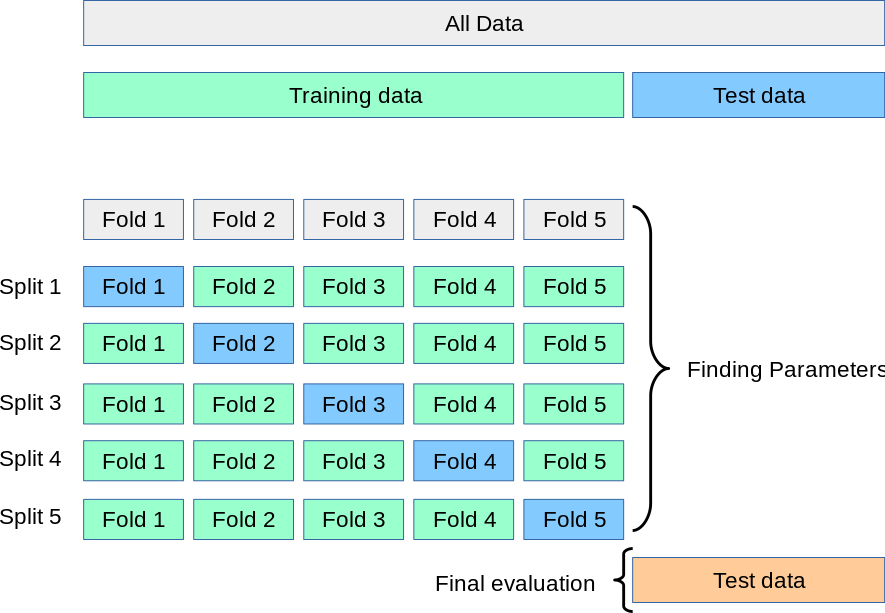
\includegraphics[scale=0.35]{figures/References/grid_search_cross_validation.png}
    \\Image from \cite{Cross-val}
    \caption{5-fold Cross-Validation}
    \label{fig:cross_validation}
\end{figure}

The grid-search method iterated through multiple combinations of \((C, \gamma)\) pairs until the pair with the best cross-validation accuracy is achieved. The parameters were varied as follows: 
\[C = [2^{-15}, 2^{-14}, 2^{-13}, ..., 2^2, 2^3]\]
\[\gamma = [2^{-15}, 2^{-14}, 2^{-13}, ..., 2^2, 2^3]\]

For this study, a 10-fold cross-validation was used in order to not overfit the training data \cite{Nagi}. Scikit-learn's built-in function GridSearchCV was used for this. After the best (\emph{C}, $\gamma$) pair was obtained, the training set was trained again using the (\emph{C}, $\gamma$) pair to obtain the final classifier. The performance of the classifier was evaluated using the testing set.

The entire training and testing procedure was repeated for each of the seven dataset categories in \ref{tab:Dataset}.

\subsection{ANN}
\label{section:sec04_03_02} 
A deep feed forward neural network inspired by \cite{Ismail} was modeled using Keras, a deep-learning API. The neural network consisted of an input layer, multiple hidden layers, and an output layer. The input layer has 63 neurons, representing the features of the dataset: 55 household meter readings and \% loss error of the 8 check meters. Let \emph{L} be the number of hidden layers and \emph{N} be the number of neurons in each of the hidden layers. The output layer has a single neuron that outputs a value of either '1', which means that theft is present, or '0', which means there is no theft present.

From Figure \ref{fig:ANNneuron}, it can be seen that for every neuron, there is a bias and a corresponding weight for every input. Let $m$ be the number of inputs to a neuron, $w_i$ as the weight of the \emph{ith} input, and $b$ as the bias value. The output of a single neuron is
\[y_{in} = b + \sum_{i=1}^{m} w_i x_i\]
An activation function maps $y_{in}$ to a range of values to produce the neuron's final output. This is calculated for all neurons of each layer, from the input layer to the output layer.

Let $W^l$ be the matrix that defines the weight of the neurons in layer \emph{l}. Likewise, let $b^l$ be the vector that defines the bias of neurons in layer \emph{l}. Training the detector means using an optimization algorithm such as stochastic gradient descent to solve for the model parameters $W^l$ and $b^l$ by minimizing the cross-entropy loss function
\begin{equation}
\min_{C} C = - \left(y_d\log{(p_d)}\right) - \left(1-y_d\right)\log{(1-p_d)}
\end{equation}
where $y_d$ is the label of data point $d$ and $p_d$ is the prediction of the model for the same data point $d$. The model described in \cite{Ismail}, which consists of a feed forward stage and a backward propagation stage every iteration, was used to solve for the optimal parameters $W^l$ and $b^l$ for every layer.

In designing neural networks, hyperparameters such as the optimizer, learning rate, activation function, and number of hidden layers and neurons, must be carefully selected such that the optimum performance is achieved \cite{Bengio}. In designing the neural network of this paper, grid-search using k-cross validation was performed to iteratively find the best combination of hyperparameters.

The subsequent sections discuss each of the hyperparameters used in training the neural network.
\begin{figure} [H]
    \centering
    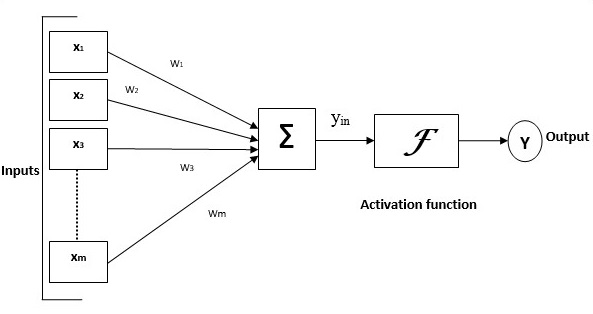
\includegraphics[scale=0.9]{figures/References/ANNneuron.jpg}
    \\Image from \cite{Neuron}
    \caption{Model of a single artificial neuron}
    \label{fig:ANNneuron}
\end{figure}

\subsubsection{Optimizer and Learning Rate}
\label{section:sec04_03_02_01}
The optimization algorithm, \(\mathcal{O}\), determines how the weights and biases of neurons in each layer are updated during the backpropagation stage. In choosing the best optimizer for the neural network, the computing time and its use in previous electricity theft detection research were considered. As such, the best optimizer was chosen between the Stochastic Gradient Descent (SGD) and Adaptive Moment Estimation (ADAM).

SGD is one of the most dominantly used optimization algorithms in deep-learning neural networks \cite{adam}. It is the preferred optimization algorithm for large datasets in which the computing time is the limiting factor rather than dataset size \cite{Montavon}. ADAM, another variant of gradient descent, is also typically used in large datasets but is more computationally efficient and requires little memory \cite{adam}.

Both of these gradient-based optimizers have a parameter \(\eta\) called \emph{learning rate}, which controls the step size or how fast the weights and biases are updated by the optimizer. Setting this too low will lead to slow training times, while setting it too high may cause divergence errors \cite{Bengio}. The learning rate is set to an initial value and gradually decreases during training. In practice, the initial learning rate is manually adjusted and depends highly on the problem, hence the need to find the optimal value through hyperparameter optimization \cite{Schaul}. 

For hyperparameter optimization, the following values were used:
\[\mathcal{O} = \{SGD, ADAM\}\]
\[\eta = \{0.1, 0.2, 0.3, 0.4, 0.5, 0.6, 0.7, 0.8, 0.9\}\]

\subsubsection{Activation Function}
\label{section:sec04_03_02_03} 
In Figure \ref{fig:ANNneuron}, an activation function, \(\mathcal{A}\), maps the output of a neuron to a range of values. In most neural networks, hidden layers use the same activation function while the activation function of the output layer highly depends on the problem. For binary classification problems, the sigmoid function is used because it maps the output to either 0 or 1.

For the hidden layers of the paper's neural network, the activation function was chosen between the sigmoid function, the hyperbolic tan function, and the Rectified Linear Unit (ReLU) function. These are the most commonly used activation functions in deep-learning models \cite{Nwankpa}. Figure \ref{fig:Activation} shows the plot of the three different activation functions.

The sigmoid function, given by
\begin{equation}
f(x) = \frac{1}{1+e^{-x}}
\end{equation}
is a zero-centered function and maps the output between 0 and 1. It is typically used in output layers of binary classification models but can also be used in hidden layers as well.

The hyperbolic tan function, given by
\begin{equation}
f(x) = \frac{e^x - e^{-x}}{e^x + e^{-x}}
\end{equation}
is similar to the sigmoid function but has a smoother center and maps the output between -1 and 1. It is reported that the hyperbolic tan function gives better training performance for multi-layer neural networks \cite{Nwankpa}.

The third activation function, ReLU, was developed in 2010 and is regarded as the most widely used activation function for hidden layers because it addressed the shortcomings of both the sigmoid and hyperbolic tan functions \cite{Nwankpa}. It is given by
\begin{equation}
f(x) = max(0,x) = \begin{cases} 
      x_i, & x\geq 0 \\
      0, & x < 0
   \end{cases}
\end{equation}

\begin{figure}[H]
    \centering
    \subfloat[\centering Sigmoid]{{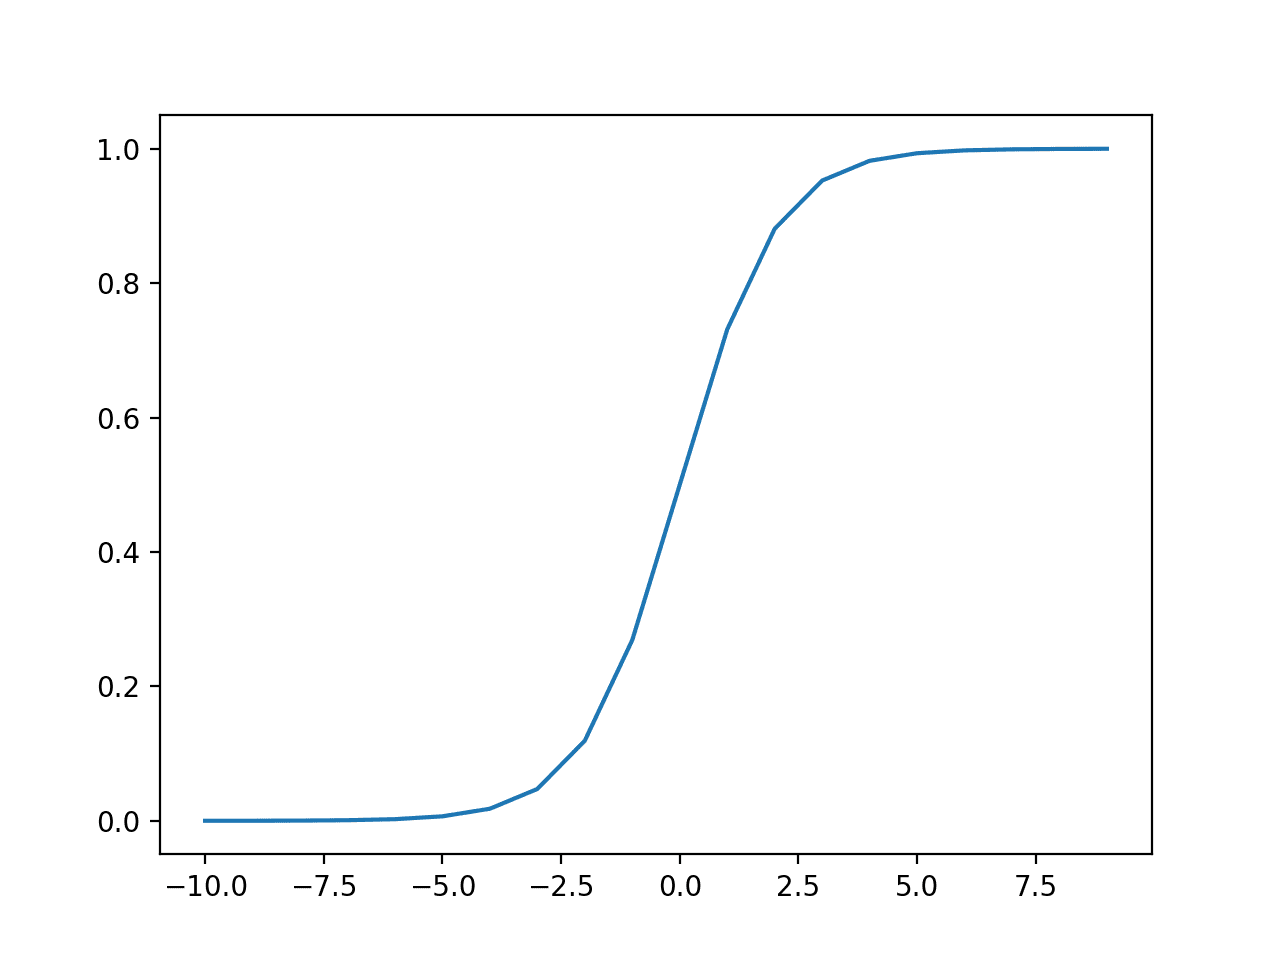
\includegraphics[width=5cm]{figures/References/sigmoid.png} }}
    \subfloat[\centering Hyperbolic Tan]{{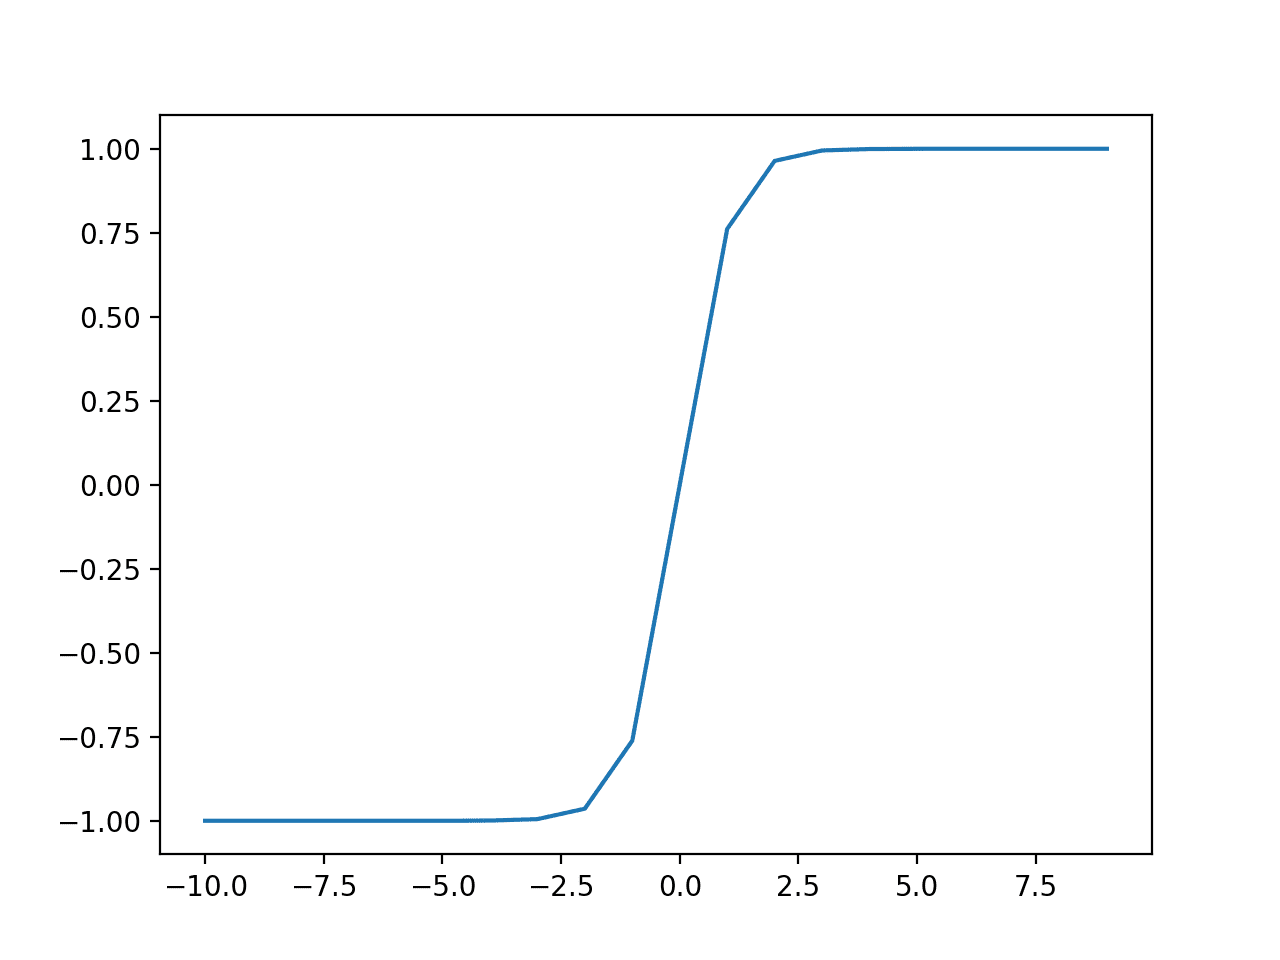
\includegraphics[width=5cm]{figures/References/tanh.png} }}
    \subfloat[\centering ReLU]{{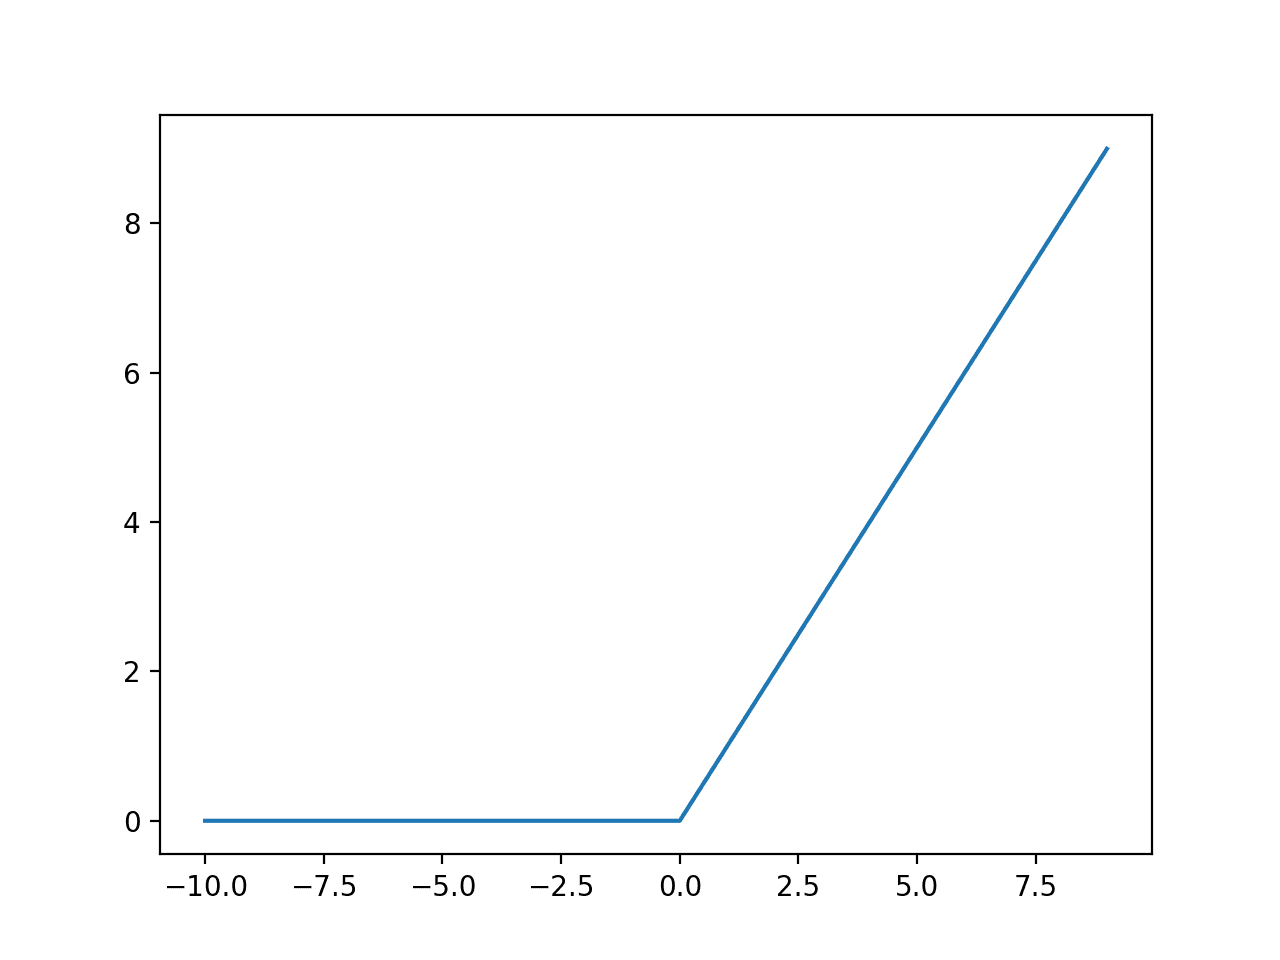
\includegraphics[width=5cm]{figures/References/relu.png} }}
    \caption{Activation Functions}
    \label{fig:Activation}
\end{figure}

For hyperparameter optimization, the following values were used:
\[\mathcal{A}_{hidden} = \{sigmoid, tanh, relu\}\]

\subsubsection{Epoch and Batch Size}
\label{section:sec04_03_02_04} 
The number of times the network trains on the training set is called epoch or \(\mathcal{E}\). Every epoch, a small subset of the training set is used to update the weights and biases of the network. The size of this subset is called batch size or \(\mathcal{B}\). Epoch and batch size are optimized together since in theory, they mostly affect training time and not necessarily performance. However, changes in epoch and batch size may affect other hyperparameters, and as such, must be optimized together with the other hyperparameters as well \cite{Bengio}.

For hyperparameter optimization, the following values were used:
\[\mathcal{E} = \{20, 50, 100\}\]
\[\mathcal{B} = \{32, 64, 128\}\]

\subsubsection{Hidden Layers and Number of Neurons}
\label{section:sec04_03_02_05}
The number of neurons, or \(n_h\), in each hidden layer, and the number of hidden layers, are directly correlated to the capacity and complexity of the neural network. For linear problems, a single hidden layer is enough, but for more complicated, non-linear problems, a network with multiple hidden layers perform better. According to \cite{Larochelle}, using the same number of neurons for all hidden layers produced better results than using different ones. 

For this neural network, the number of hidden layers was set to 3. The number of neurons of each hidden layer was set to values approaching the maximum number of neurons in the input layers, as in \cite{Mukherjee}.

For hyperparameter optimization, the following values were used:
\[n_h  = \{20, 40, 60\}\]

\subsubsection{\emph{K}-fold Cross-Validation}
\label{section:sec04_03_02_06}
The datasets were standardized to a normalized scale such that the data have zero mean and unit variance. Each dataset category in Table \ref{tab:Dataset} was split 80:20 into training and testing sets.

Similar to Section \ref{section:sec04_03_01}, \emph{k}-fold cross-validation was used to find the best performing combination of the hyperparameters discussed. Accuracy was used as the scoring criterion.

Figure \ref{fig:ANNLayers} illustrates the neural network model to be optimized. The number written in a layer denotes the number of neurons in that layer. The following summarizes all the hyperparameters that were optimized using a 10-fold cross-validation procedure:
\begin{equation} \label{equation:hyperparameters}
\begin{split}
& \mathcal{O} = \{SGD, ADAM\} \\
& \eta = \{0.1, 0.2, 0.3, 0.4, 0.5, 0.6, 0.7, 0.8, 0.9\} \\
& \mathcal{A}_{hidden} = \{sigmoid, tanh, relu\} \\
& \mathcal{E} = \{20, 50, 100\} \\
& \mathcal{B} = \{32, 64, 128\} \\
& n_h  = \{20, 40, 60\} 
\end{split}
\end{equation}
After obtaining the best performing combination of the hyperparameters, the training set was trained again using the chosen hyperparameters to obtain the final classifier. Finally, the performance of the classifier was evaluated using the testing set. The entire neural network was made using the Sequential model function from Keras.

The entire training and testing procedure was repeated for each of the dataset categories in \ref{tab:Dataset}.

\begin{figure} [H]
    \centering
    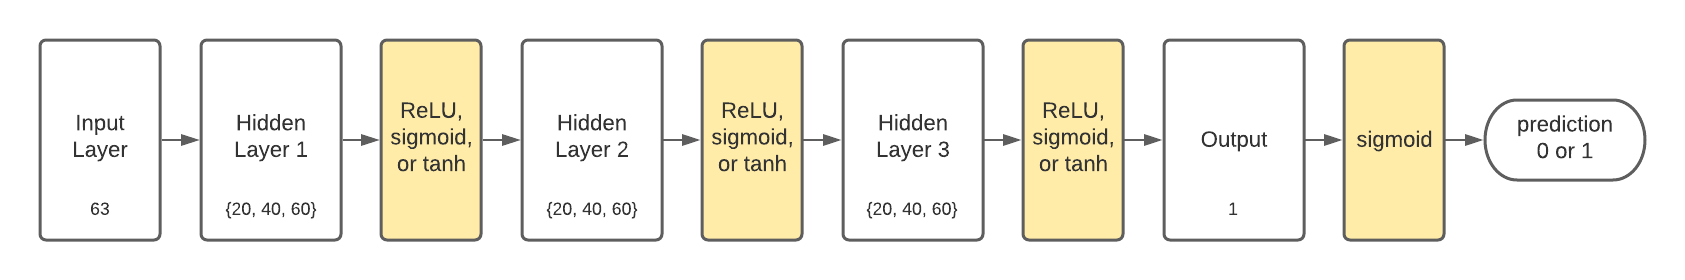
\includegraphics[scale=0.6]{figures/References/Layers.png}
    \caption{Theft Detection Neural Network Model}
    \label{fig:ANNLayers}
\end{figure}

\subsection{Anomaly Coefficient Calculation}
\label{section:sec04_03_03} 

Anomaly Coefficient Calculation describes the use of coincident meter measurements and writes them as sets of linear equations to detect pilferage \cite{MendiolaPedrasa}. By solving the linear equations, the algorithm derives a set of coefficients that is multiplied to each household meter and identifies the pilferer by analyzing the coefficients. The parameters are given by the coincident smart meter readings of the households and their respective check meter. The computed coefficients determine the factor by which the pilferer scaled its meter readings. The algorithm was originally tested on a test system where all customers are equipped with smart meters, and a check meter is connected upstream to measure the total consumption of the network.  

A set of linear equations that are derived from Equation \eqref{equation:GeneralEqAC} can be formed from the check meter and household meter readings, which can be represented as a matrix equation \(C = MK\). From the equation, having {\it N} meter readings would require {\it N} equations to solve for their respective anomaly coefficients {\it k}. The coefficients may be solved using matrix inversion if the matrix is square similar to Equation  \eqref{equation:MatrixInvAC}. Constrained least squares method is used if there are insufficient meter readings from a given system. Since a gathered time frame data could be less than the variables under study in a large test network, this method minimizes the errors in producing such coefficients for the system. 

\begin{equation}
\label{equation:GeneralEqAC}
CM_t = {M_{at}k_a + M_{bt}k_b + ....\,M_{nt}k_n}
\end{equation}

Where:
\\
\indent\(CM_t\) = check meter reading at time \(t\)
\\
\indent\(M_{xt}\) = meter reading of customer \(x\) at time \(t\)
\\
\indent\(k_xt\) = anomaly coefficient of customer \(x\)

\begin{equation}
\label{equation:MatrixInvAC}
\begin{bmatrix}
k_a\\
k_b\\
k_c\\
\vdots\\
k_x\\
\end{bmatrix}=
\begin{bmatrix}
M_{a1} & M_{b1} & M_{c1} & \dots & M_{x1}\\
M_{a2} & M_{b2} & M_{c2} &\dots & M_{x2}\\
M_{a3} & M_{b3} & M_{c3} & \dots & M_{x3}\\
\vdots & \vdots & \vdots & \ddots & \\
M_{at} & M_{bt} & M_{ct} & \dots & M_{xt}\\
\end{bmatrix}^{-1} \times
\begin{bmatrix}
CM_1\\
CM_2\\
CM_3\\
\vdots\\
CM_t\\
\end{bmatrix}
\end{equation}

Constrained least squares was used in this project since each data point has 48 time frames only, which is insufficient for a system with 55 households. Since {\it t}, number of time frames where theft occurs, is less than that of {\it x}, number of households inside the check meter, matrix inversion would be unable to solve for the corresponding coefficients of each household. 

Constrained least square is the process of solving for {\it k} that may satisfy Equation \ref{equation:SubjectTo}. The upper and lower limits of the constraints used in this method is solved by using Equation \ref{equation:kAnomaly} and inputting a maximum {\it m} value of 0.65, which is the maximum value of \(k_{et}\) derived from Section \ref{section:sec04_02_04}, and minimum {\it m} value of 0, in which there is no pilferage in the system. Using these constraints, the coefficients of each household can be solved while limiting it to an upper limit of 2.86 and a lower limit of 1.  It is important to note that since there are not enough time frames to perform matrix inversion, the results may differ in cases wherein there are sufficient time frames.

\begin{equation}
\label{equation:SubjectTo}
MIN\norm{Ak - b}^2
\end{equation}

Where:
\\
\indent\(A\) = matrix for the set of household readings
\\
\indent\(k\) = anomaly coefficient matrix
\\
\indent\(b\) = matrix of CM readings

\begin{equation}
\label{equation:kAnomaly}
k = \frac{1}{1+m}
\end{equation}

Where:
\\
\indent\(+m\) means that the meter is recording \textbf{more} than expected
\\
\indent\(-m\) means that the meter is recording \textbf{less} than expected
\\

Given that there are sufficient time frames to work with, and there is no pilferer in the system, all the {\it k} in the equation will have a value close to one given that there is zero or minimal loss in the system. This means that the sum of all the smart meter readings is equal to the check meter reading. If a pilferer is present, their corresponding {\it k} will be greater than 1; this is illustrated in Equation \ref{equation:kAnomaly}, and shown in Figure \ref{fig:kAnomalyValues}.

In a real life setup, technical losses that are present in the system affect the error between the check meter and household meter readings. Because of this, the check meter readings may differ from the sum of the downstream households. Additionally, when the pilferage occurs at a very short duration, its effect on the system may be insignificant enough for the pilferer to be detected since the algorithms relies on the number of time frames with theft.

\begin{figure}[H]
    \centering
    \subfloat[\centering {\it k} Without Pilferage]{{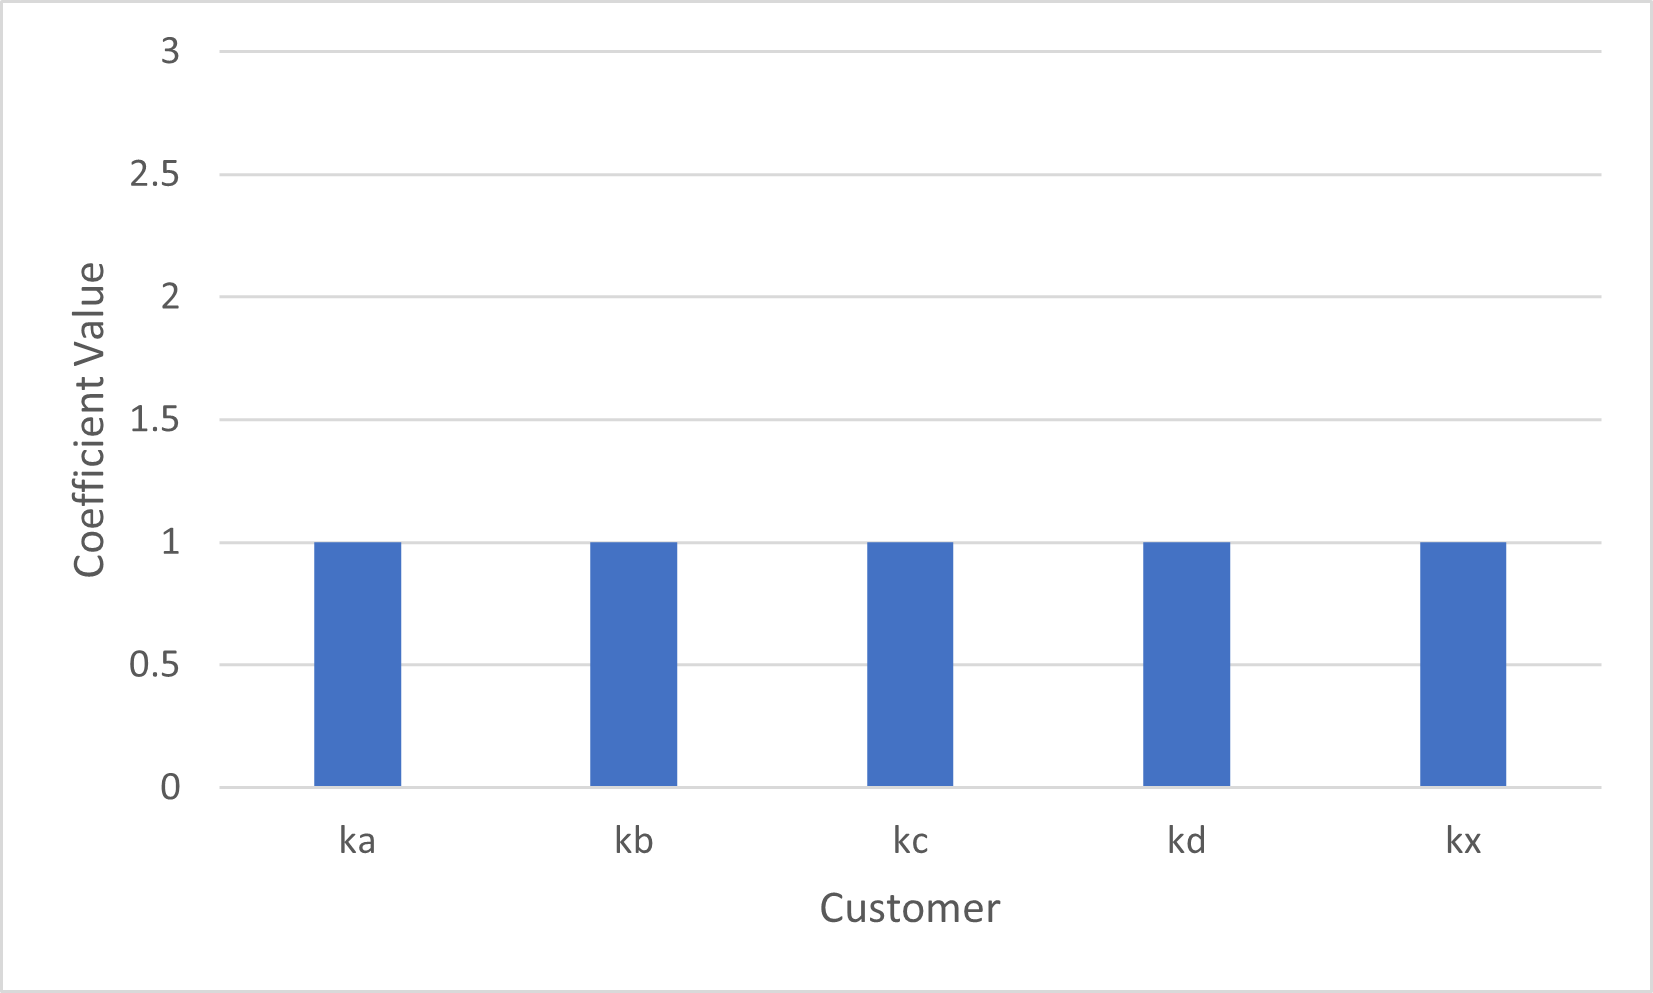
\includegraphics[width=7cm]{figures/References/Anomaly_kBen.png}}}
    \qquad
    \subfloat[\centering {\it k} With Pilferage]{{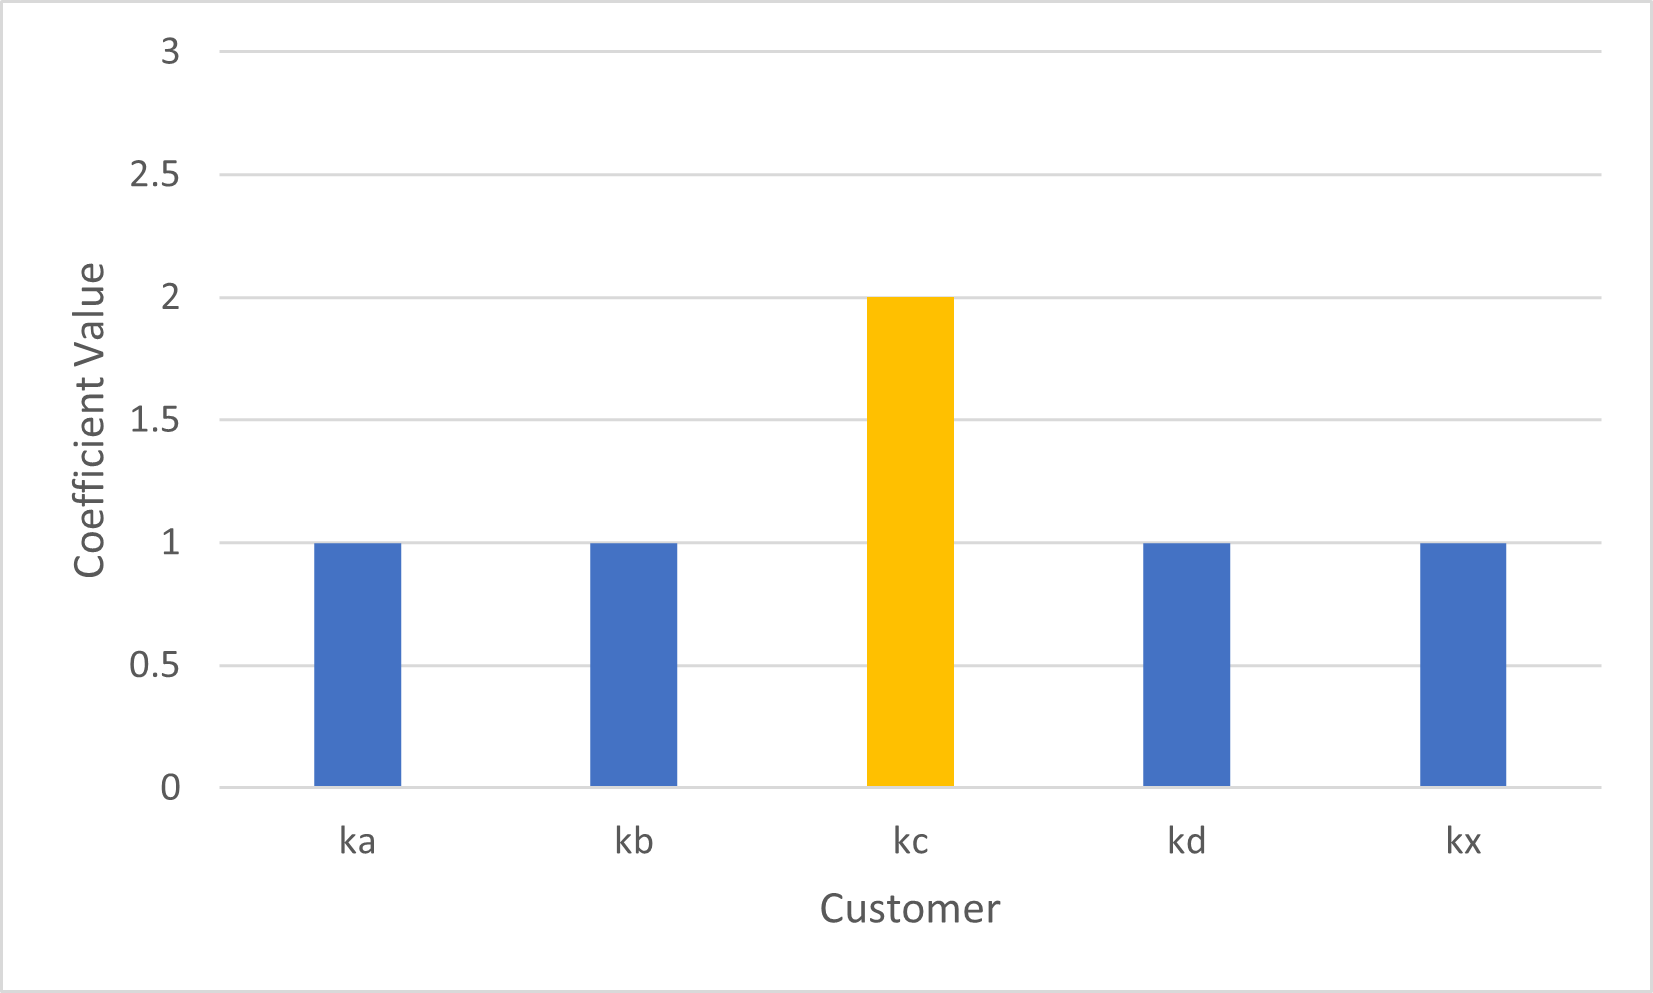
\includegraphics[width=7cm]{figures/References/Anomaly_kMal.png}}}
    \caption{Coefficient {\it k} Values}
    \label{fig:kAnomalyValues}
\end{figure}

The algorithm's performance was tested using the datasets that were created in Section \ref{section:sec04_02}. Similar to \cite{MendiolaPedrasa}, there is also one pilferer in each simulation of the created datasets. To highlight the effect of Net Metering and rooftop PVs on the the algorithm, the time frames wherein there is no pilferage present were removed. This is because inclusion of time frames with no pilferage will disturb the natural coefficient of each household as shown by \cite{MendiolaPedrasa}. For theft frequency B, these are the time frames outside 6AM to 6PM. Additionally, only the main check meter shown in Section \ref{section:sec04_02_05_02} was used to replicate the original process done in \cite{MendiolaPedrasa}. Since there are 55 households and only 48 time frames, constrained least squares method was used to solve for the {\it k} values. 

To identify the pilferer in the system, the calculated {\it k} value of each household were compared to a threshold value. The pilferer is identified if its {\it k} value is larger than the threshold value. Setting the threshold value is a crucial part of the algorithm, and significantly affects its ability to correctly detect and identify the pilferer. 

Because of this, multiple thresholds were considered and tested. The different thresholds were computed based on the possible values of \(k_{et}\) in Section \ref{section:sec04_02_04} and the Equation \ref{equation:kAnomaly}. If there are multiple {\it k} values that are larger than the threshold, the largest {\it k} and its corresponding household was predicted to be the pilferer. 

The outputs of this algorithm are: whether or not  there is pilferage in the system, and the household number of the pilferer.

\section{Performance Metrics Calculation}
\label{section:sec04_04}

For binary classification models, a two-by-two confusion matrix determines the four possible outcomes of the predicted value of the classifier. From the confusion matrix in \ref{tab:Confusion Matrix}, the four measures that can be obtained are: True Positive (TP) and True Negative (TN), which are the number of correctly predicted positive and negative cases, and False Positive (FP) and False Negative (FN), which refers to the number of wrongly predicted positive and negative cases \cite{Maamar}\cite{Seliya}.


\begin{table}[H]
\centering
\begin{tabular}{|
>{\columncolor[HTML]{FFFFFF}}l |
>{\columncolor[HTML]{FFFFFF}}l |
>{\columncolor[HTML]{FFFFFF}}l |}
\hline
\multicolumn{1}{|c|}{\cellcolor[HTML]{FFFFFF}{\color[HTML]{333333} }}                               & \multicolumn{2}{c|}{\cellcolor[HTML]{FFFFFF}\textbf{Predicted Value}}                                                                    \\ \cline{2-3} 
\multicolumn{1}{|c|}{\multirow{-2}{*}{\cellcolor[HTML]{FFFFFF}{\color[HTML]{333333} \textbf{Actual Value}}}} & \textbf{Positive}                                                       & \textbf{Negative}                                                       \\ \hline
Positive                                                                                            & \begin{tabular}[c]{@{}l@{}}True Positive \\ (TP)\end{tabular}  & \begin{tabular}[c]{@{}l@{}}False Negative \\ (FP)\end{tabular} \\ \hline
Negative                                                                                            & \begin{tabular}[c]{@{}l@{}}False Positive \\ (FP)\end{tabular} & \begin{tabular}[c]{@{}l@{}}True Negative \\ (TN)\end{tabular}  \\ \hline
\end{tabular}
\caption{\label{tab:Confusion Matrix}Confusion Matrix}
\end{table}

For evaluating the theft detection and theft identification algorithms, accuracy, precision, recall, and F1 scores were used. These metrics were the ones considered on whether Rooftop PV and Net Metering can significantly affect the performance of electricity theft detection and identification algorithms.

\subsection{Accuracy}
\label{section:sec04_04_01}

This gives the ratio of correctly predicted observations (TP + TN) to the total observations. While accuracy is a great way of determining outright the best model, the symmetry of the datasets is also to be considered. Accuracy works best for datasets that are symmetric where values of false positives (FP) and false negatives (FN) are almost the same \cite{Uddin}. The formula for accuracy is given by

\begin{equation}
\label{equation:Accuracy}
Accuracy = \frac{TP+TN}{TP+FP+FN+TN}
\end{equation}

\subsection{Precision}
\label{section:sec04_04_02}

This is the ratio of correctly predicted positive observations (TP) to the total predicted positive observations, may it be correct (TP) or incorrect (FP). High scores of precision relate to a low false positive rate. Precision can be seen as a measure of the quality of the classifier. The formula for precision is given by

\begin{equation}
\label{equation:Precision}
Precision = \frac{TP}{TP+FP}
\end{equation}

\subsection{Recall}
\label{section:sec04_04_03}

Recall, sometimes referred to as sensitivity, determines the ratio of correctly predicted positive observations (TP) to all actual positives (TP + FN). High recall means that an algorithm returns most of the relevant results, whether or not irrelevant ones are also returned. Unlike the precision metric earlier, this is more of a quantity measurement of the classifier. The formula for recall is given by

\begin{equation}
\label{equation:Recall}
Recall = \frac{TP}{TP+FN}
\end{equation}

\subsection{F1}
\label{section:sec04_04_04}

F1 is the weighted average of Precision and Recall. This gives us a more in-depth result than the Accuracy as it takes into account both false positive (FP) and false negative (FN). This is usually a better metric especially if false positive (FP) and false negative (FN) do not bear the same weight, especially on datasets that are not symmetric \cite{Uddin}. The formula for F1 score is given by

\begin{equation}
\label{equation:F1}
F1 Score = \frac{2(DR \cdot PR)}{DR+PR}
\end{equation}

\cleardoublepage{}

%%%%%%%%%%%%%%%%%%%%%%%%%%%%%%%%%%%%%%%%%%%%%%%%%%%%%%%%%%%%%%%%%
\chapter{Results and Discussions\label{cha:chap05}}

\section{Theft Detection Algorithm Results}
\label{section:sec05_01}

\subsection{SVM Results}
After performing 10-fold cross-validation on the training sets of each dataset category, the \((C, \gamma)\) pairs with the highest accuracy scores were selected. The optimum parameter pairs of each dataset category are presented in Table \ref{tab:SVMParameters}. 

\label{section:sec05_01_01}
\begin{table}[H]
\centering
\begin{tabular}{|l|c|c|}
\hline
\multicolumn{1}{|c|}{\textbf{Dataset}} & \multicolumn{1}{c|}{\textbf{C}} & \multicolumn{1}{c|}{\textbf{$\gamma$}} \\ \hline
D1 (0\% PV)                             & 8                               & 0.015625                               \\ \hline
D2 (20\% PV)                            & 8                               & 0.015625                               \\ \hline
D3 (70\% PV)                            & 8                               & 0.0078125                              \\ \hline
D4 (20\% PV, 20\% NM)                   & 8                               & 0.0078125                              \\ \hline
D5 (20\% PV, 70\% NM)                   & 8                               & 0.0078125                              \\ \hline
D6 (70\% PV, 20\% NM)                   & 8                               & 0.0078125                              \\ \hline
D7 (70\% PV, 70\% NM)                   & 8                               & 0.0078125                              \\ \hline
\end{tabular}
\caption{\label{tab:SVMParameters}SVM Parameter Results}
\end{table}

Using the optimized parameters, the classifiers were trained again on the training set and evaluated on the testing set of each dataset category. Since there is an element of randomness during the training stage, testing and training were repeated 6 times per dataset and the average of its performance metrics were recorded. Table \ref{tab:SVM} presents the final performance metrics of each dataset using an SVM classifier. A single run of training and testing took approximately 12 minutes.

\begin{table}[H]
\centering
\begin{tabular}{|l|r|r|r|r|}
\hline
\multicolumn{1}{|c|}{\textbf{Dataset}} &
  \multicolumn{1}{c|}{\textbf{Accuracy}} &
  \multicolumn{1}{c|}{\textbf{Precision}} &
  \multicolumn{1}{c|}{\textbf{Recall}} &
  \multicolumn{1}{c|}{\textbf{F1}} \\ \hline
D1 (0\% PV)           & 0.9708 & 0.9989 & 0.9426 & 0.9699 \\ \hline
D2 (20\% PV)          & 0.9654 & 0.9943 & 0.9361 & 0.9643 \\ \hline
D3 (70\% PV)          & 0.9275 & 0.9819 & 0.8712 & 0.9230 \\ \hline
D4 (20\% PV, 20\% NM) & 0.9156 & 0.9772 & 0.8517 & 0.9097 \\ \hline
D5 (20\% PV, 70\% NM) & 0.8312 & 0.9340 & 0.7132 & 0.8078 \\ \hline
D6 (70\% PV, 20\% NM) & 0.7549 & 0.8792 & 0.5909 & 0.7054 \\ \hline
D7 (70\% PV, 70\% NM) & 0.5985 & 0.6724 & 0.3842 & 0.4881 \\ \hline
\end{tabular}
\caption{\label{tab:SVM}SVM Results}
\end{table}

\begin{figure} [H]
    \centering
    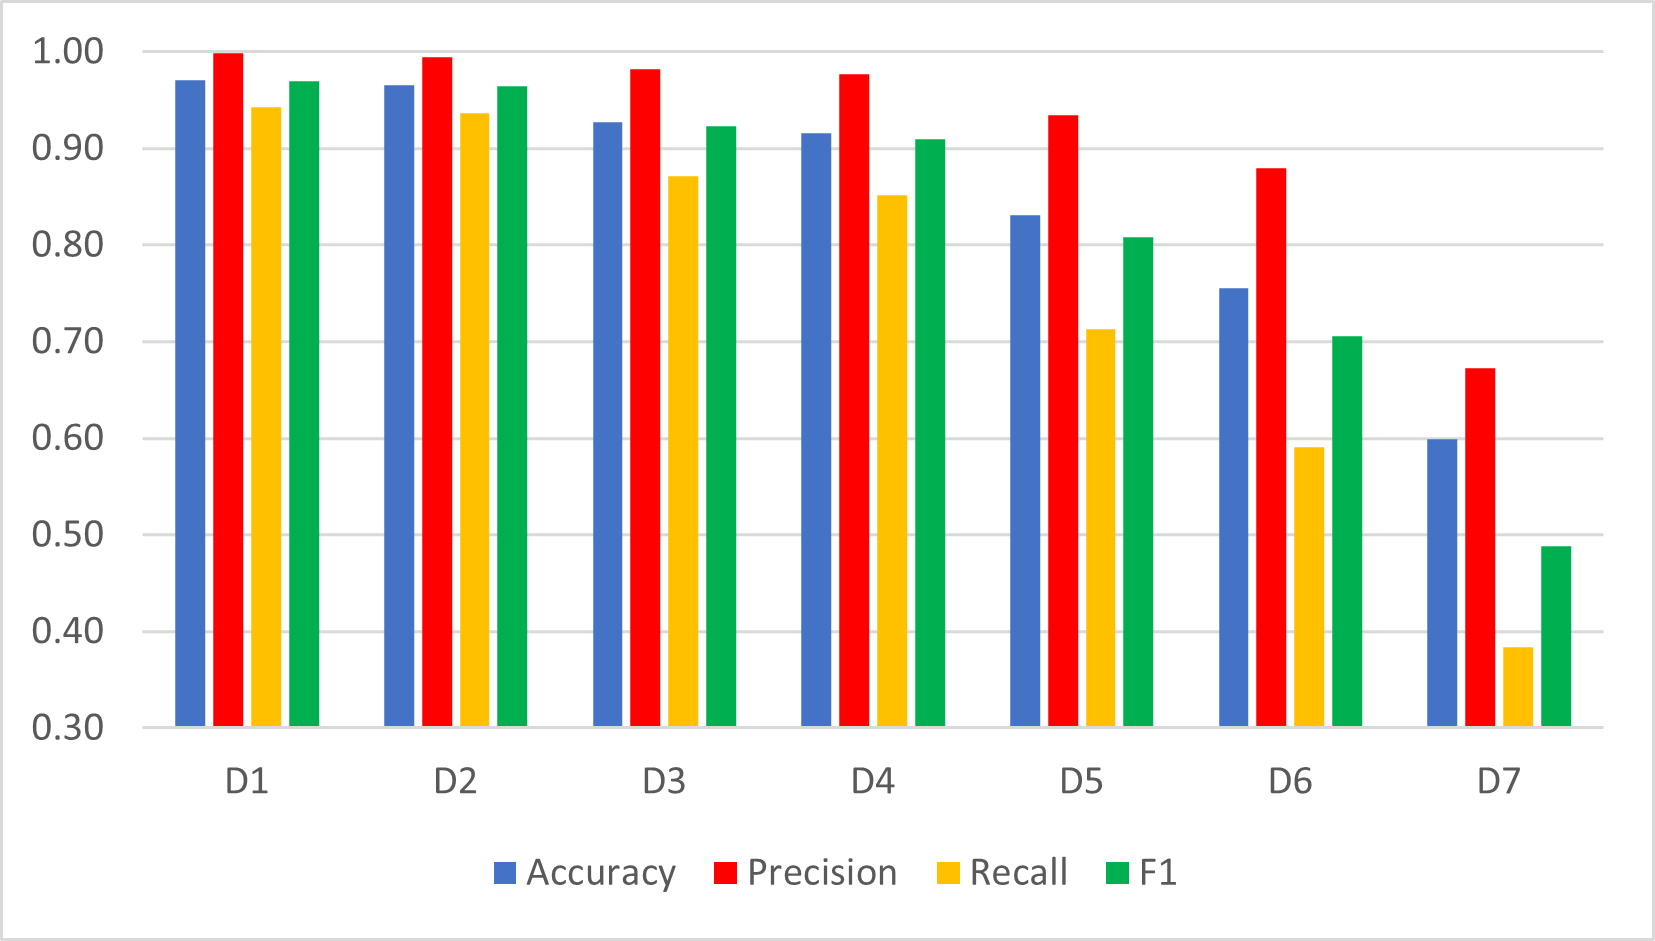
\includegraphics[scale=0.8]{figures/ResultBarGraphs/SVM/SVM_D1to7.png}
    \caption{SVM Results - Dataset 1 to 7 Graph}
    \label{fig:SVM1to7}
\end{figure}

The average accuracy across all datasets is 85.20\%, which shows that the SVM classifier can successfully detect electricity theft given the meter readings of each household and the \% loss error of each check meter. Dataset 1 has the highest metric scores with an accuracy of 97.08\%, while Dataset 7 has the lowest with an accuracy of 59.85\%. Figure \ref{fig:SVM1to7} presents the overall trend across the datasets. The graph shows that as the number of households with rooftop PV and Net Metering increases, the metric scores worsen.

\begin{figure} [H]
    \centering
    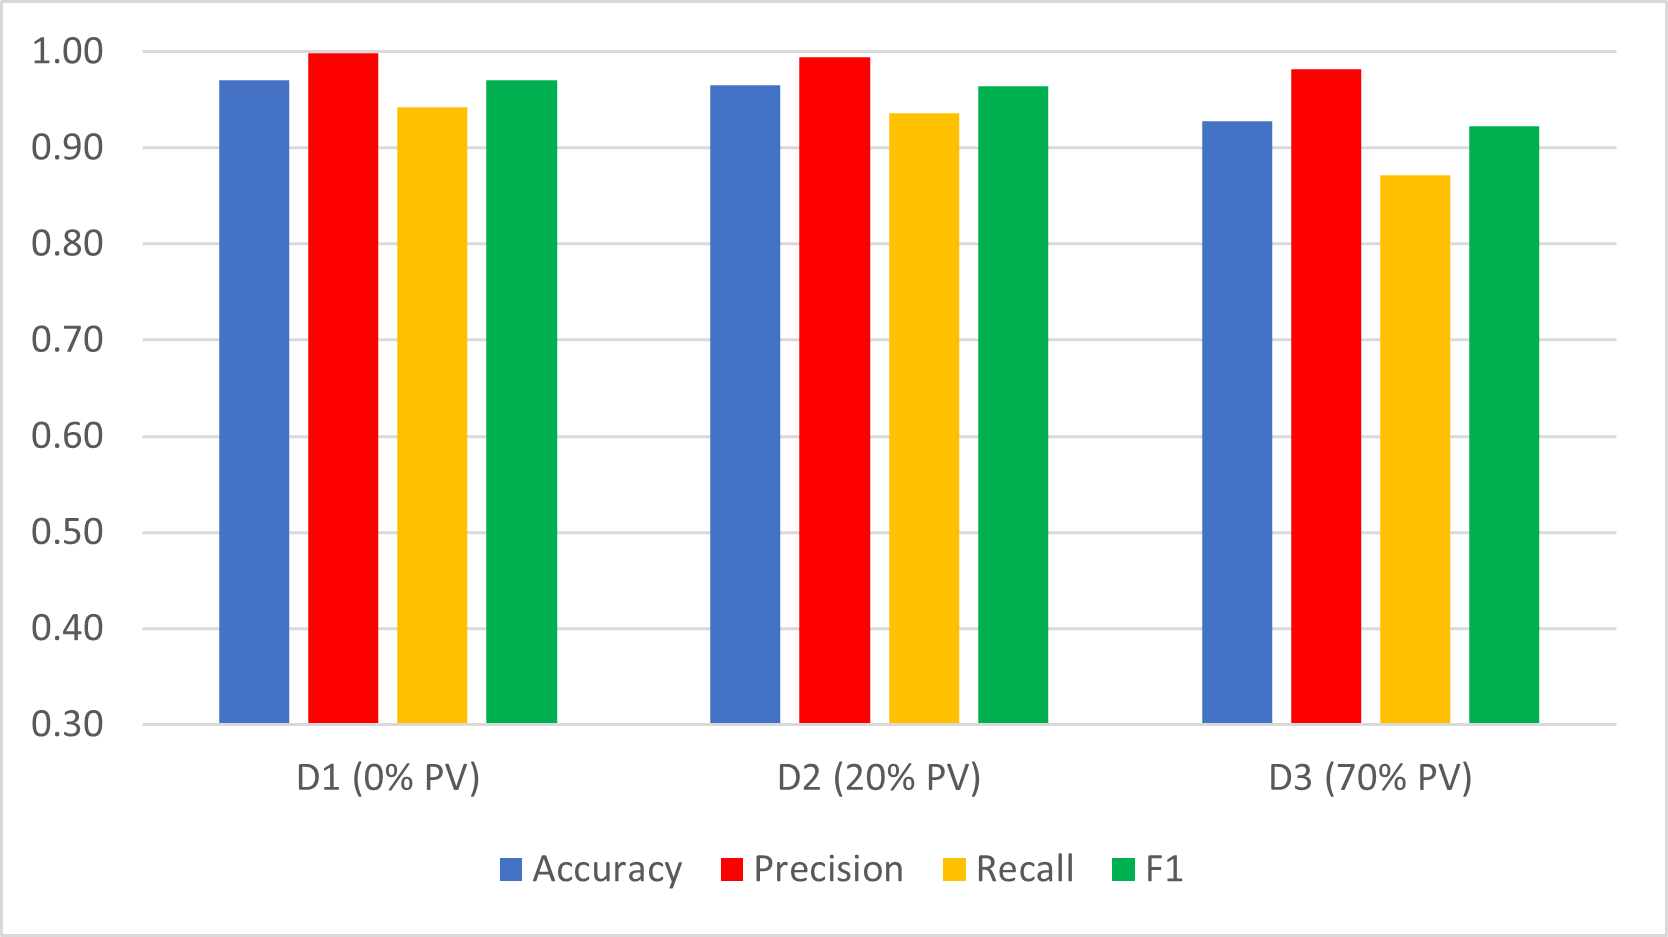
\includegraphics[scale=0.8]{figures/ResultBarGraphs/SVM/SVM_D123.png}
    \caption{SVM Results - Varying PV Penetration Graph}
    \label{fig:SVM123}
\end{figure}

Figure \ref{fig:SVM123} compares Datasets 1, 2, and 3, which has varying PV penetration and no Net Metering. The metric scores of these datasets have very close values, with the accuracy scores having a low standard deviation of 1.93\%. Despite having very close values, there is still a slightly noticeable downward trend in classifier performance as PV penetration is increased.

\begin{figure}[H]
    \centering
    \subfloat[\centering 20\% PV Penetration]{{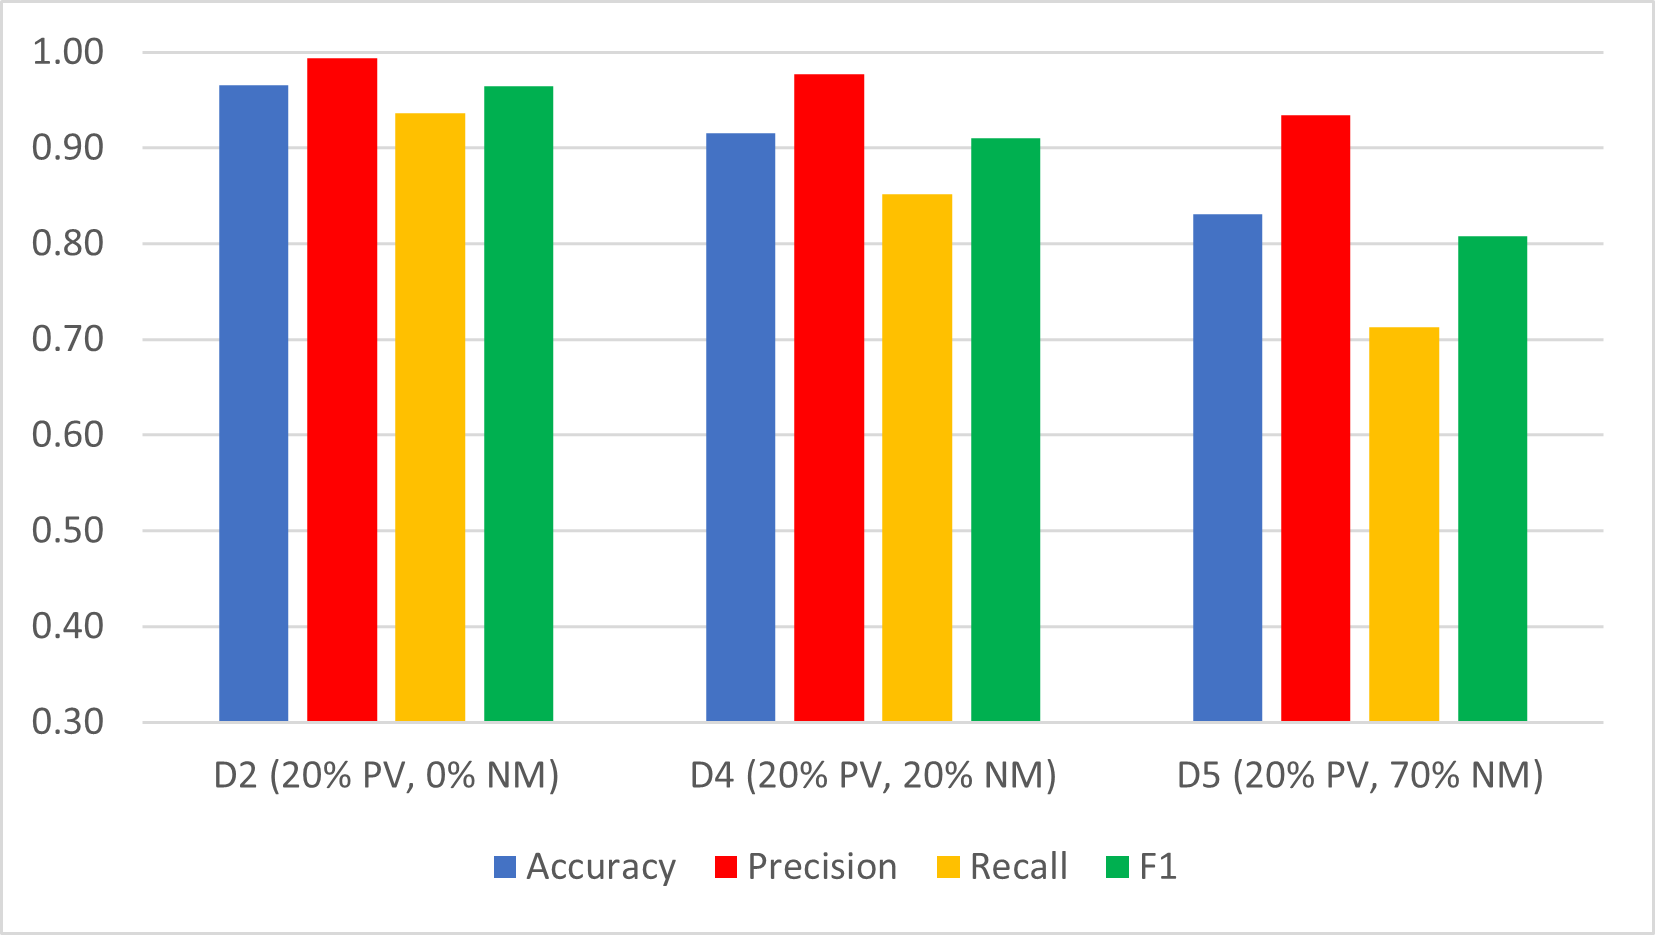
\includegraphics[width=8.2cm]{figures/ResultBarGraphs/SVM/SVM_D245.png} }}
    \subfloat[\centering 70\% PV Penetration]{{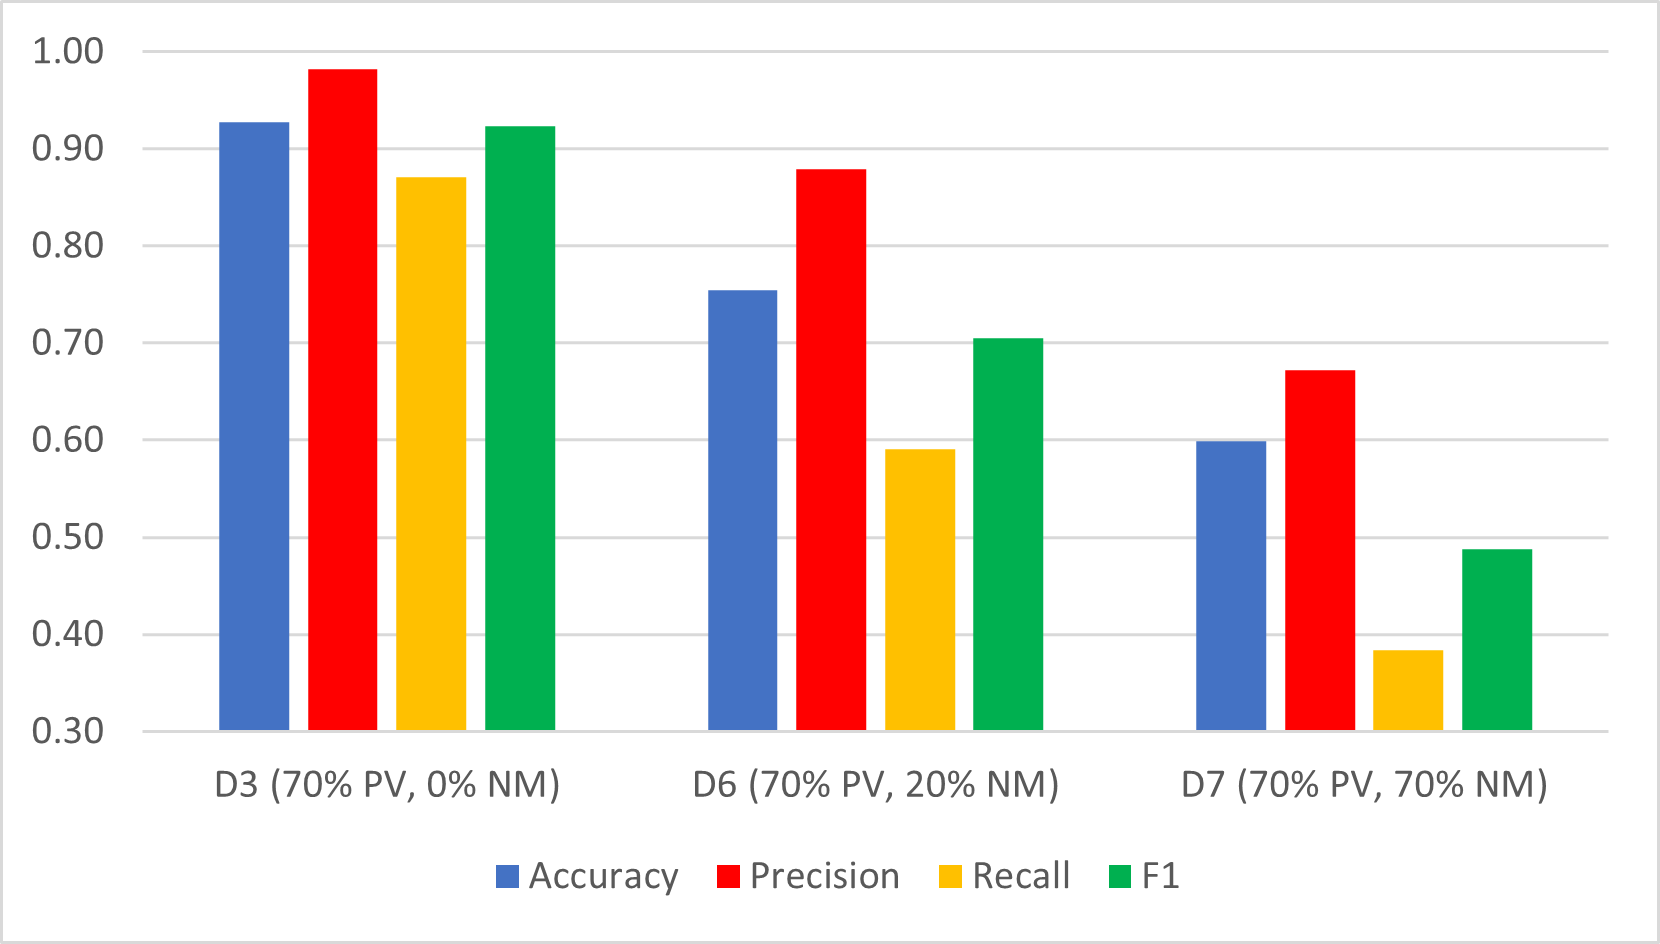
\includegraphics[width=8.2cm]{figures/ResultBarGraphs/SVM/SVM_D367.png} }}
    \caption{SVM Results - Constant PV Penetration with Varying NM Penetration Graph}
    \label{fig:SVM245367}
\end{figure}

Figures \ref{fig:SVM245367} presents the datasets in which the PV penetration is held constant at 20\% and 70\% respectively, while the NM penetration is varied. At a constant 20\% PV penetration, there is very noticeable downward trend as Net Metering penetration is increased. The accuracy scores of Dataset 2, 4, and 5, have a standard deviation of 5.54\%. This is slightly higher than when only the PV penetration is varied and there is no Net Metering present. When the PV penetration is increased to 70\%, the downward trend becomes steeper as the Net Metering penetration is varied; the standard deviation of the accuracy scores increased to 13.44\%. To illustrate, given a network with 55 households and at 20\% PV and 20\% Net Metering, the number of households with PV is \(\lfloor55\times0.2\rfloor=11\) and the number of households with both PV and Net Metering is \(\lfloor11\times0.2\rfloor=2\). At 70\% PV and 20\% Net Metering, the households with PV is now \(\lfloor55\times0.7\rfloor=38\) and the number of households with both PV and Net Metering is \(\lfloor38\times0.2\rfloor=11\). Because the number of households with PV increased drastically at 70\% PV penetration, the effect of Net Metering is amplified, hence the worsened metrics scores.

Based on the simulation results, adding rooftop PV and Net Metering to a network has a conclusive effect on the performance of SVM electricity theft detectors that primarily use household meter readings and check meter \% loss error as features. The difference between a worst-case scenario network having a majority of its households with both rooftop PV and Net Metering, and a network with no rooftop PV at all, is very significant. Between Datasets 1 and 7, accuracy drastically dropped by 37.23\%. If having an accuracy of 80\% is used as the standard in evaluating a classifier as effective, then using SVM on a network with up to 20\% of its households installed with rooftop PV and up to 70\% of those installed with Net Metering, will produce successful predictions. Further increasing the penetration of both PV and Net Metering worsens the capability of the classifier to detect electricity theft.

\subsection{ANN Results}
\label{section:sec05_01_02}
Presented in Table \ref{tab:ANNParameters} are the optimized hyperparameters of the neural network for each of the datasets after performing 10-fold cross-validation. Almost all of the datasets picked SGD as the best optimizer except Dataset 6 and 7. For the hidden layer activation function, ReLU was picked for all datasets. All the datasets, except Dataset 1, took 100 epochs until the best accuracy score was achieved. Dataset 1 trained considerably faster; it only took 50 epochs for it to achieve its best accuracy score. Dataset 7 has the highest learning rate, \(\eta\), at 0.9, which made sense since its batch size \(\mathcal{B}\) is also the highest at 128. Higher batch sizes typically require faster learning rates to achieve the same accuracy score \cite{Bengio}.

\begin{table}[H]
\centering
\begin{tabular}{|c|c|c|c|c|c|c|}
\hline
\textbf{Dataset} & \textbf{$\mathcal{O}$} & \textbf{$\eta$} & \textbf{$\mathcal{A}_{hidden}$} & \textbf{$\mathcal{E}$} & \textbf{$\mathcal{B}$} & \textbf{$n_h$} \\ \hline
1                & SGD        & 0.1        & ReLU       & 50         & 32         & 60          \\ \hline
2                & SGD        & 0.1        & ReLU       & 100        & 64         & 40          \\ \hline
3                & SGD        & 0.1        & ReLU       & 100        & 64         & 40          \\ \hline
4                & SGD        & 0.1        & ReLU       & 100        & 64         & 40          \\ \hline
5                & SGD        & 0.1        & ReLU       & 100        & 32         & 60          \\ \hline
6                & ADAM       & 0.3        & ReLU       & 100        & 64         & 60          \\ \hline
7                & ADAM       & 0.9        & ReLU       & 100        & 128        & 60          \\ \hline
\end{tabular}
\caption{\label{tab:ANNParameters}ANN Optimized Hyperparameters}
\end{table}

\begin{table}[H]
\centering
\begin{tabular}{|
>{\columncolor[HTML]{FFFFFF}}l |
>{\columncolor[HTML]{FFFFFF}}r |
>{\columncolor[HTML]{FFFFFF}}r |
>{\columncolor[HTML]{FFFFFF}}r |
>{\columncolor[HTML]{FFFFFF}}r |}
\hline
\multicolumn{1}{|c|}{\cellcolor[HTML]{FFFFFF}\textbf{Dataset}} & \multicolumn{1}{c|}{\cellcolor[HTML]{FFFFFF}\textbf{Accuracy}} & \multicolumn{1}{c|}{\cellcolor[HTML]{FFFFFF}\textbf{Precision}} & \multicolumn{1}{c|}{\cellcolor[HTML]{FFFFFF}\textbf{Recall}} & \multicolumn{1}{c|}{\cellcolor[HTML]{FFFFFF}\textbf{F1}} \\ \hline
D1 (0\% PV)
                                                            & 0.9800                                                         & 0.9978                                                          & 0.9621                                                       & 0.9796                                                   \\ \hline
D2 (20\% PV)                                                            & 0.9735                                                         & 0.9814                                                          & 0.9654                                                       & 0.9733                                                   \\ \hline
D3 (70\% PV)                                                            & 0.9226                                                         & 0.9264                                                          & 0.9199                                                       & 0.9225                                                   \\ \hline
D4 (20\% PV, 20\% NM)                                                            & 0.9188                                                         & 0.9387                                                          & 0.8961                                                       & 0.9169                                                   \\ \hline
D5 (20\% PV, 70\% NM)                                                            & 0.8696                                                         & 0.8814                                                          & 0.8571                                                       & 0.8679                                                   \\ \hline
D6 (70\% PV, 20\% NM)                                                            & 0.8009                                                         & 0.8413                                                          & 0.7435                                                       & 0.7885                                                   \\ \hline
D7 (70\% PV, 70\% NM)                                                            & 0.6374                                                         & 0.6856                                                          & 0.5238                                                       & 0.5874                                                   \\ \hline
\end{tabular}
\caption{\label{tab:ANN}ANN Results}
\end{table}

After obtaining the optimum hyperparameters for each dataset, the classifiers were trained again on the training set and evaluated using the testing set. This was performed 6 times per dataset and the average of the performance metrics were recorded. Table \ref{tab:ANN} shows the measured performance metrics of each dataset. The neural network was modeled in Keras and training and testing time took approximately 8 minutes per run.

The results show that all datasets except Dataset 7 have accuracy scores above 80\%. The average accuracy across all datasets using a neural network classifier is 87.18\%, with a standard deviation of 11.13\%. It is worth noting that the base case, Dataset 1, has almost perfect metric scores. Its precision is almost 100\%, signifying that false positive outcomes are very rare. Additionally, its recall is less than the precision, which tells us that making a false negative is more common than making a false positive. This is satisfactory because it is less possible for the distribution utility company to accuse innocent customers.

\begin{figure} [H]
    \centering
    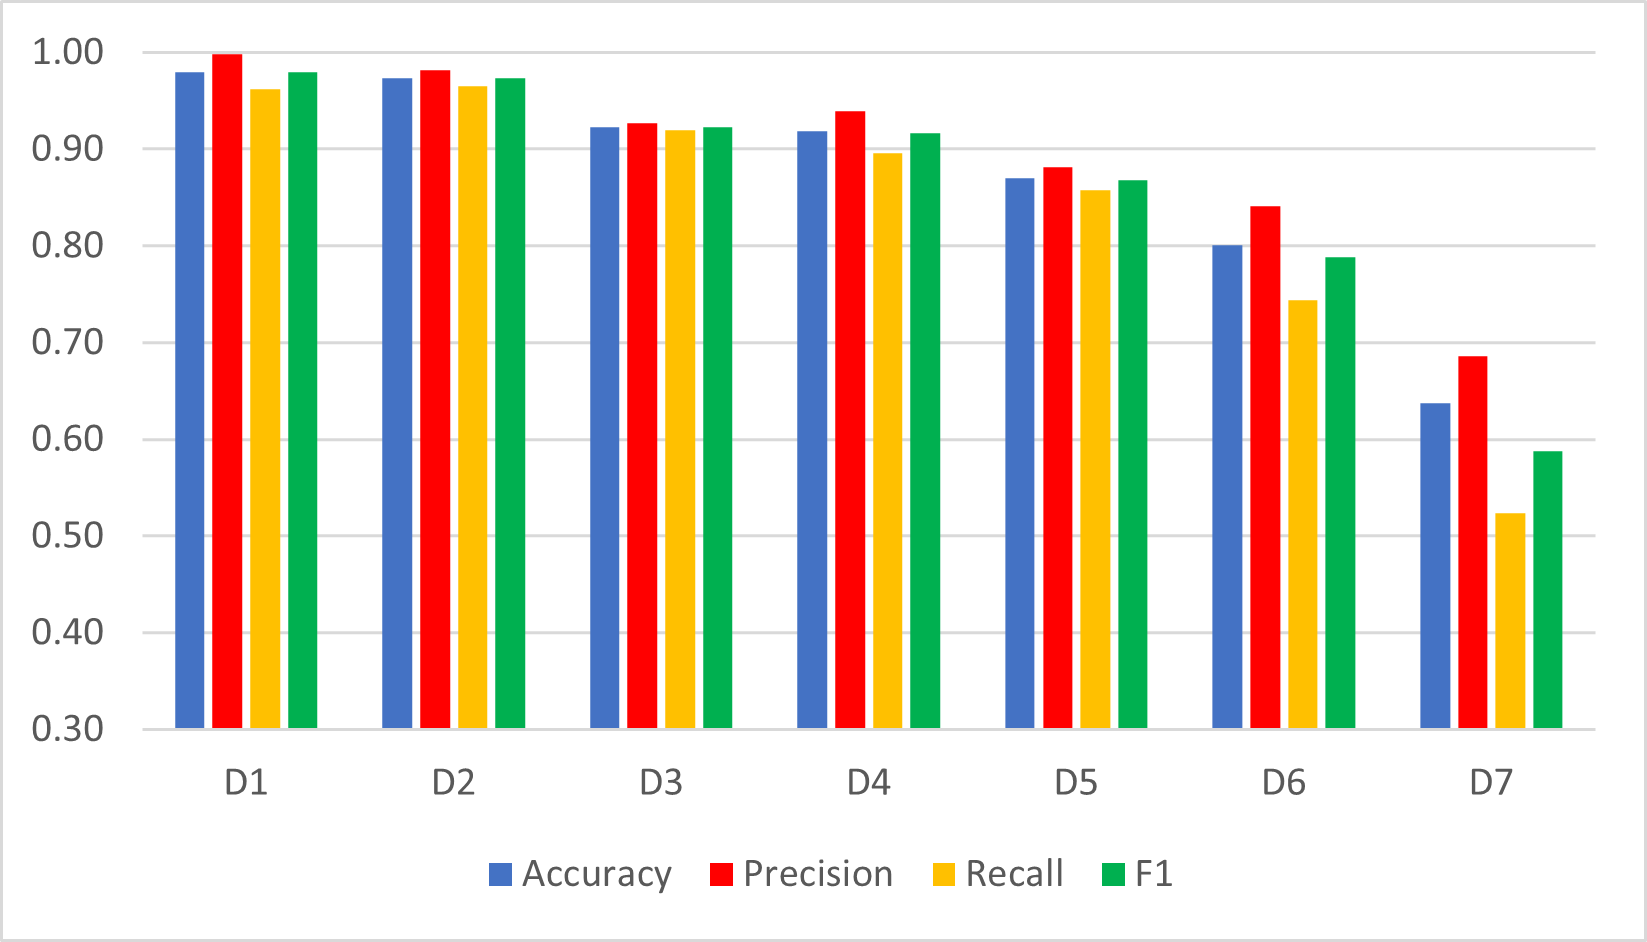
\includegraphics[scale=0.8]{figures/ResultBarGraphs/ANN/ANN_D1to7.png}
    \caption{ANN Results - Dataset 1 to 7 Graph}
    \label{fig:ANN1to7}
\end{figure}

\begin{figure} [H]
    \centering
    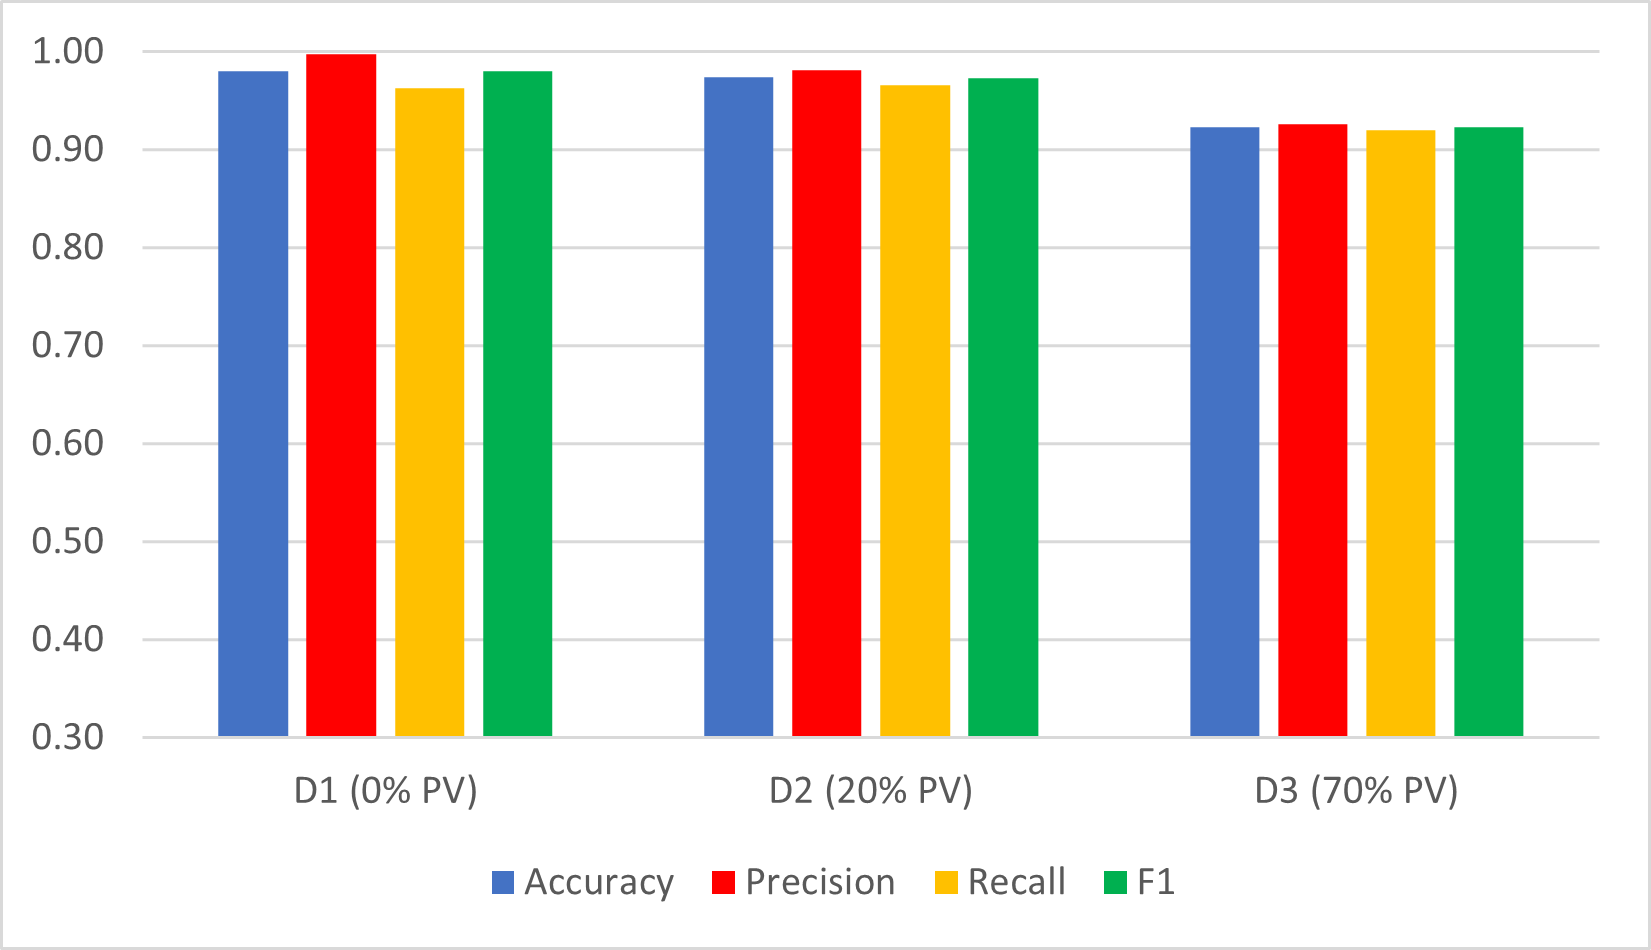
\includegraphics[scale=0.8]{figures/ResultBarGraphs/ANN/ANN_D123.png}
    \caption{ANN Results - Varying PV Penetration Graph}
    \label{fig:ANN123}
\end{figure}

The overall trend of the performance metrics across datasets is highlighted in Figure \ref{fig:ANN1to7}. Datasets 1, 2, 3 and 4, have high metric scores above 90\%, while Dataset 7 has the worst scores. The recall of Dataset 7 is 52.38\%, which is alarming because it signifies that it has a high number of false negative predictions. A pilferer would have the best chances of staying undetected in a network with a majority of its households installed with both PV and Net Metering.

Figure \ref{fig:ANN123} shows that at varying PV penetration with no Net Metering, the difference in the metric scores is minimal. On the other hand, Figure \ref{fig:ANN245367} shows that if PV penetration is held constant and we vary the number of households with Net Metering, the metric scores decrease significantly. The effect of Net Metering is more apparent in Figure \ref{fig:ANN245367_B} since the base number of households with PV is higher (70\% PV penetration). Therefore, Net Metering has a worse effect on the performance of a neural network classifier than the presence of PV alone.

\begin{figure}[H]
    \centering
    \subfloat[\centering 20\% PV Penetration \label{fig:ANN245367_A}]{{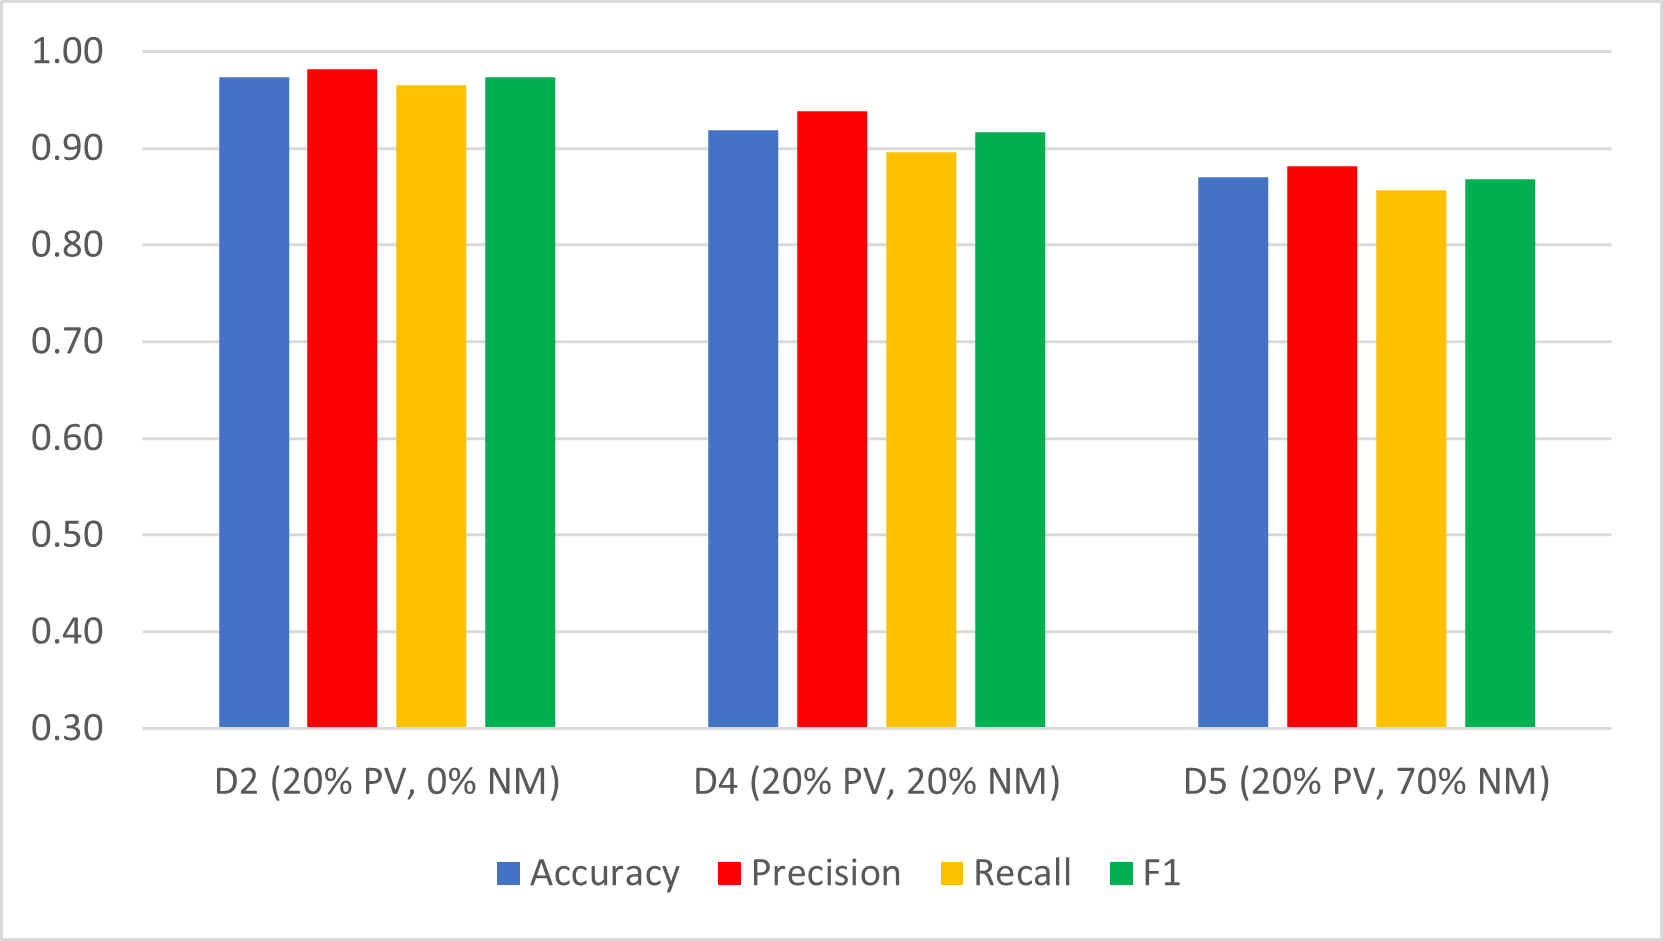
\includegraphics[width=8.2cm]{figures/ResultBarGraphs/ANN/ANN_D245.png} }}
    \subfloat[\centering 70\% PV Penetration \label{fig:ANN245367_B}]{{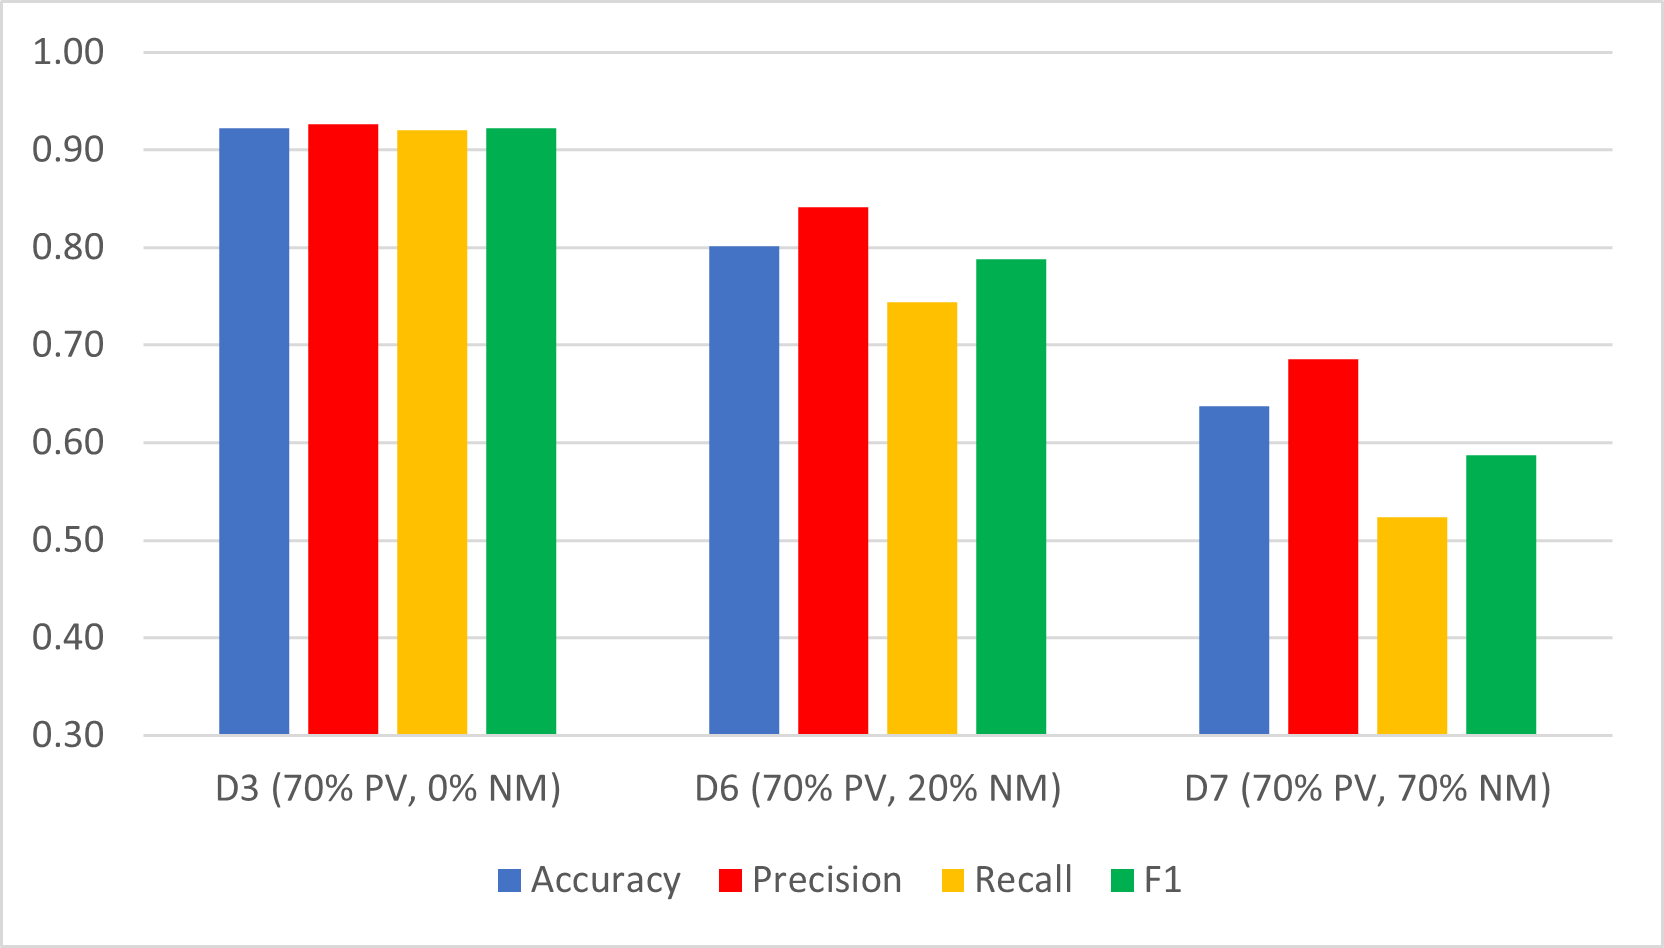
\includegraphics[width=8.2cm]{figures/ResultBarGraphs/ANN/ANN_D367.png} }}
    \caption{ANN Results - Constant PV Penetration with Varying NM Penetration Graph}
    \label{fig:ANN245367}
\end{figure}

Based on the results of the simulations, it is evident that a neural network classifier trained using a dataset with household meter readings and \% loss error as its features, will perform exceptionally in detecting electricity theft, provided that the majority of the households do not have both PV and Net Metering installed. As the number households with Net Metering increases, performance of the classifier worsens especially at high PV penetration.

It is worth noting that the results of the SVM classifier is very similar to that of the ANN classifier. The overall trend across varying levels of PV and Net Metering penetration is the same on both types of classifiers: detection performance has a negative relationship with PV and Net Metering penetration. The similarity in the results can be attributed to the fact that both types of classifiers used the same dataset with the same features. As such, it is necessary to examine the characteristics of the dataset and its features to identify the cause of the decreasing trend.

\subsection{Anomaly Coefficient Calculation Results}
\label{section:sec05_01_03}

Anomaly Coefficient Calculation identifies the household where the theft occurs unlike SVM and ANN. Because of this, its confusion matrix is different from the confusion matrix of SVM and ANN. The way to determine a True Positive, True Negative, False Positive, or False Negative is given by:
\begin{itemize}
  \item TP, if the algorithm correctly predicts that there is theft and identifies the right pilferer.
  \item TN, if the algorithm correctly predicts that there is no theft.
  \item FP, if the algorithm correctly predicts that there is theft, but identifies the wrong pilferer. Or, the algorithm wrongly predicts that there is theft but there is no theft.
  \item FN, if the algorithm wrongly predicts that there is no theft but there is theft.
\end{itemize}

To make sure that the best threshold was selected for each dataset, its value was varied and the resulting performance metrics were compared with each other. The threshold 1.25 gave the highest accuracy, precision, recall and F1 score. 

Since the simulations with theft frequency B have less time frames where theft occurs, it was suspected that the algorithm may perform poorly when it is tested on this part of the dataset. With regards to this, the seven datasets were split into two subsets to further check the accuracy of the algorithm when different frequencies are tested. Three different testing data were used: the original dataset with frequencies A and B, the subset with frequency A, and the subset with frequency B.

With a threshold of 1.25, the results were recorded and tabulated. The tables are separated with respect to the included data per test. Tables \ref{tab:ACBF}, \ref{tab:ACFA}, and \ref{tab:ACFB} show the metric scores of each case. Shown below in Figure \ref{fig:ACBF}, \ref{fig:ACFA}, and \ref{fig:ACFB} are the bar graph results of the tables.

\cleardoublepage{}

\begin{table}[H]
\begin{tabular}{|
>{\columncolor[HTML]{FFFFFF}}l |
>{\columncolor[HTML]{FFFFFF}}r |
>{\columncolor[HTML]{FFFFFF}}r |
>{\columncolor[HTML]{FFFFFF}}r |
>{\columncolor[HTML]{FFFFFF}}r |}
\hline
\multicolumn{1}{|c|}{\cellcolor[HTML]{FFFFFF}\textbf{Dataset}} & \multicolumn{1}{c|}{\cellcolor[HTML]{FFFFFF}\textbf{Accuracy}} & \multicolumn{1}{c|}{\cellcolor[HTML]{FFFFFF}\textbf{Precision}} & \multicolumn{1}{c|}{\cellcolor[HTML]{FFFFFF}\textbf{Recall}} & \multicolumn{1}{c|}{\cellcolor[HTML]{FFFFFF}\textbf{F1}} \\ \hline
D1 (0\% PV)                                                            & 0.8429                                                         & 0.8159                                                          & 0.8208                                                       & 0.8183                                                   \\ \hline
D2 (20\% PV)                                                            & 0.8273                                                         & 0.7703                                                          & 0.8262                                                       & 0.7973                                                   \\ \hline
D3 (70\% PV)                                                            & 0.8318                                                         & 0.7737                                                          & 0.8571                                                       & 0.8133                                                   \\ \hline
D4 (20\% PV, 20\% NM)                                                            & 0.7935                                                         & 0.7311                                                          & 0.7756                                                       & 0.7527                                                   \\ \hline
D5 (20\% PV, 70\% NM)                                                            & 0.8513                                                         & 0.8368                                                          & 0.8258                                                       & 0.8312                                                   \\ \hline
D6 (70\% PV, 20\% NM)                                                            & 0.8266                                                         & 0.7527                                                          & 0.8729                                                       & 0.8083                                                   \\ \hline
D7 (70\% PV, 70\% NM)                                                            & 0.8422                                                         & 0.7945                                                          & 0.8618                                                       & 0.8268                                                   \\ \hline
\end{tabular}
\caption{\label{tab:ACBF}Anomaly Coefficient Calculation Results (Both Frequencies)}
\end{table}

\begin{table}[H]
\begin{tabular}{|
>{\columncolor[HTML]{FFFFFF}}l |
>{\columncolor[HTML]{FFFFFF}}r |
>{\columncolor[HTML]{FFFFFF}}r |
>{\columncolor[HTML]{FFFFFF}}r |
>{\columncolor[HTML]{FFFFFF}}r |}
\hline
\multicolumn{1}{|c|}{\cellcolor[HTML]{FFFFFF}\textbf{Dataset}} & \multicolumn{1}{c|}{\cellcolor[HTML]{FFFFFF}\textbf{Accuracy}} & \multicolumn{1}{c|}{\cellcolor[HTML]{FFFFFF}\textbf{Precision}} & \multicolumn{1}{c|}{\cellcolor[HTML]{FFFFFF}\textbf{Recall}} & \multicolumn{1}{c|}{\cellcolor[HTML]{FFFFFF}\textbf{F1}} \\ \hline
D1A (0\% PV)                                                            & 0.9506                                                         & 0.9777                                                          & 0.9213                                                       & 0.9486                                                   \\ \hline
D2A (20\% PV)                                                            & 0.9351                                                         & 0.9605                                                          & 0.9043                                                       & 0.9315                                                   \\ \hline
D3A (70\% PV)                                                            & 0.9468                                                         & 0.9616                                                          & 0.9286                                                       & 0.9448                                                   \\ \hline
D4A (20\% PV, 20\% NM)                                                            & 0.9273                                                         & 0.9793                                                          & 0.8711                                                       & 0.9220                                                   \\ \hline
D5A (20\% PV, 70\% NM)                                                            & 0.9338                                                         & 0.9883                                                          & 0.8779                                                       & 0.9298                                                   \\ \hline
D6A (70\% PV, 20\% NM)                                                            & 0.9416                                                         & 0.9538                                                          & 0.9261                                                       & 0.9398                                                   \\ \hline
D7A (70\% PV, 70\% NM)                                                            & 0.9364                                                         & 0.9563                                                          & 0.9138                                                       & 0.9346                                                   \\ \hline
\end{tabular}
\caption{\label{tab:ACFA}Anomaly Coefficient Calculation Results (Frequency A)}
\end{table}

\begin{table}[H]
\begin{tabular}{|
>{\columncolor[HTML]{FFFFFF}}l |
>{\columncolor[HTML]{FFFFFF}}r |
>{\columncolor[HTML]{FFFFFF}}r |
>{\columncolor[HTML]{FFFFFF}}r |
>{\columncolor[HTML]{FFFFFF}}r |}
\hline
\multicolumn{1}{|c|}{\cellcolor[HTML]{FFFFFF}\textbf{Dataset}} & \multicolumn{1}{c|}{\cellcolor[HTML]{FFFFFF}\textbf{Accuracy}} & \multicolumn{1}{c|}{\cellcolor[HTML]{FFFFFF}\textbf{Precision}} & \multicolumn{1}{c|}{\cellcolor[HTML]{FFFFFF}\textbf{Recall}} & \multicolumn{1}{c|}{\cellcolor[HTML]{FFFFFF}\textbf{F1}} \\ \hline
D1B (0\% PV)                                                            & 0.7351                                                         & 0.6278                                                          & 0.6855                                                       & 0.6554                                                   \\ \hline
D2B (20\% PV)                                                            & 0.7195                                                         & 0.5631                                                          & 0.7121                                                       & 0.6289                                                   \\ \hline
D3B (70\% PV)                                                            & 0.7169                                                         & 0.5852                                                          & 0.7607                                                       & 0.6615                                                   \\ \hline
D4B (20\% PV, 20\% NM)                                                            & 0.6597                                                         & 0.4722                                                          & 0.6270                                                       & 0.5387                                                   \\ \hline
D5B (20\% PV, 70\% NM)                                                            & 0.7688                                                         & 0.6807                                                          & 0.7584                                                       & 0.7175                                                   \\ \hline
D6B (70\% PV, 20\% NM)                                                            & 0.7117                                                         & 0.5579                                                          & 0.7970                                                       & 0.6563                                                   \\ \hline
D7B (70\% PV, 70\% NM)                                                            & 0.7481                                                         & 0.6319                                                          & 0.7931                                                       & 0.7034                                                   \\ \hline
\end{tabular}
\caption{\label{tab:ACFB}Anomaly Coefficient Calculation Results (Frequency B)}
\end{table}

\cleardoublepage{}

\begin{figure} [H]
    \centering
    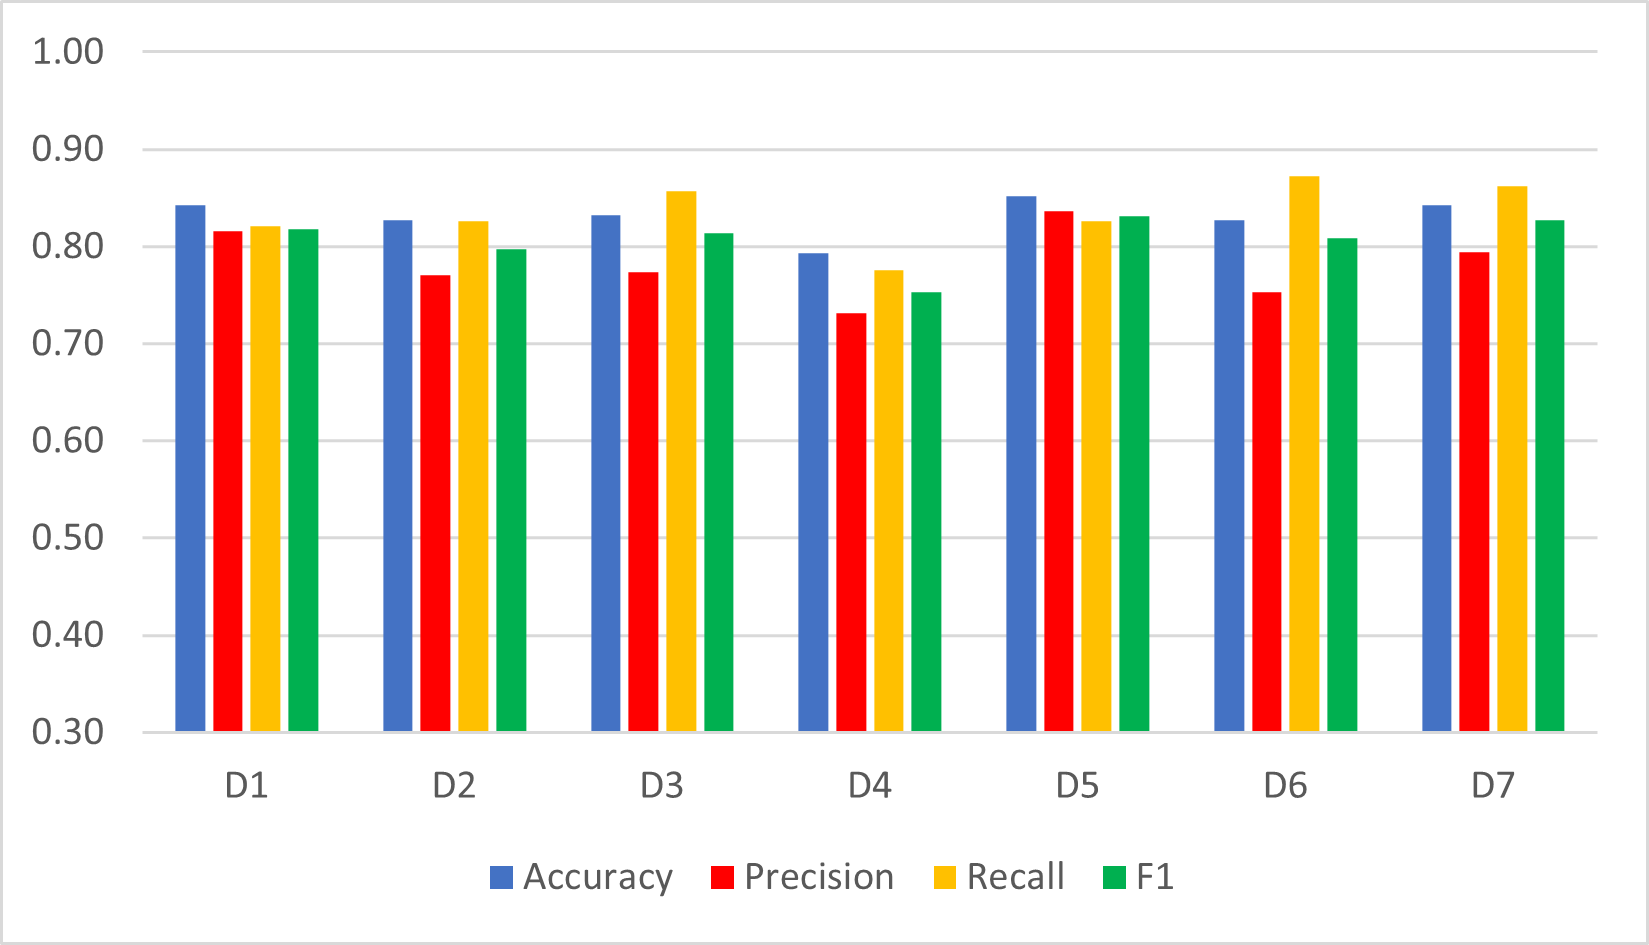
\includegraphics[scale=0.8]{figures/ResultBarGraphs/Anomaly/AC_BothFreqs.png}
    \caption{Anomaly Coefficient Calculation Graph (Both Frequencies)}
    \label{fig:ACBF}
\end{figure}

\begin{figure} [H]
    \centering
    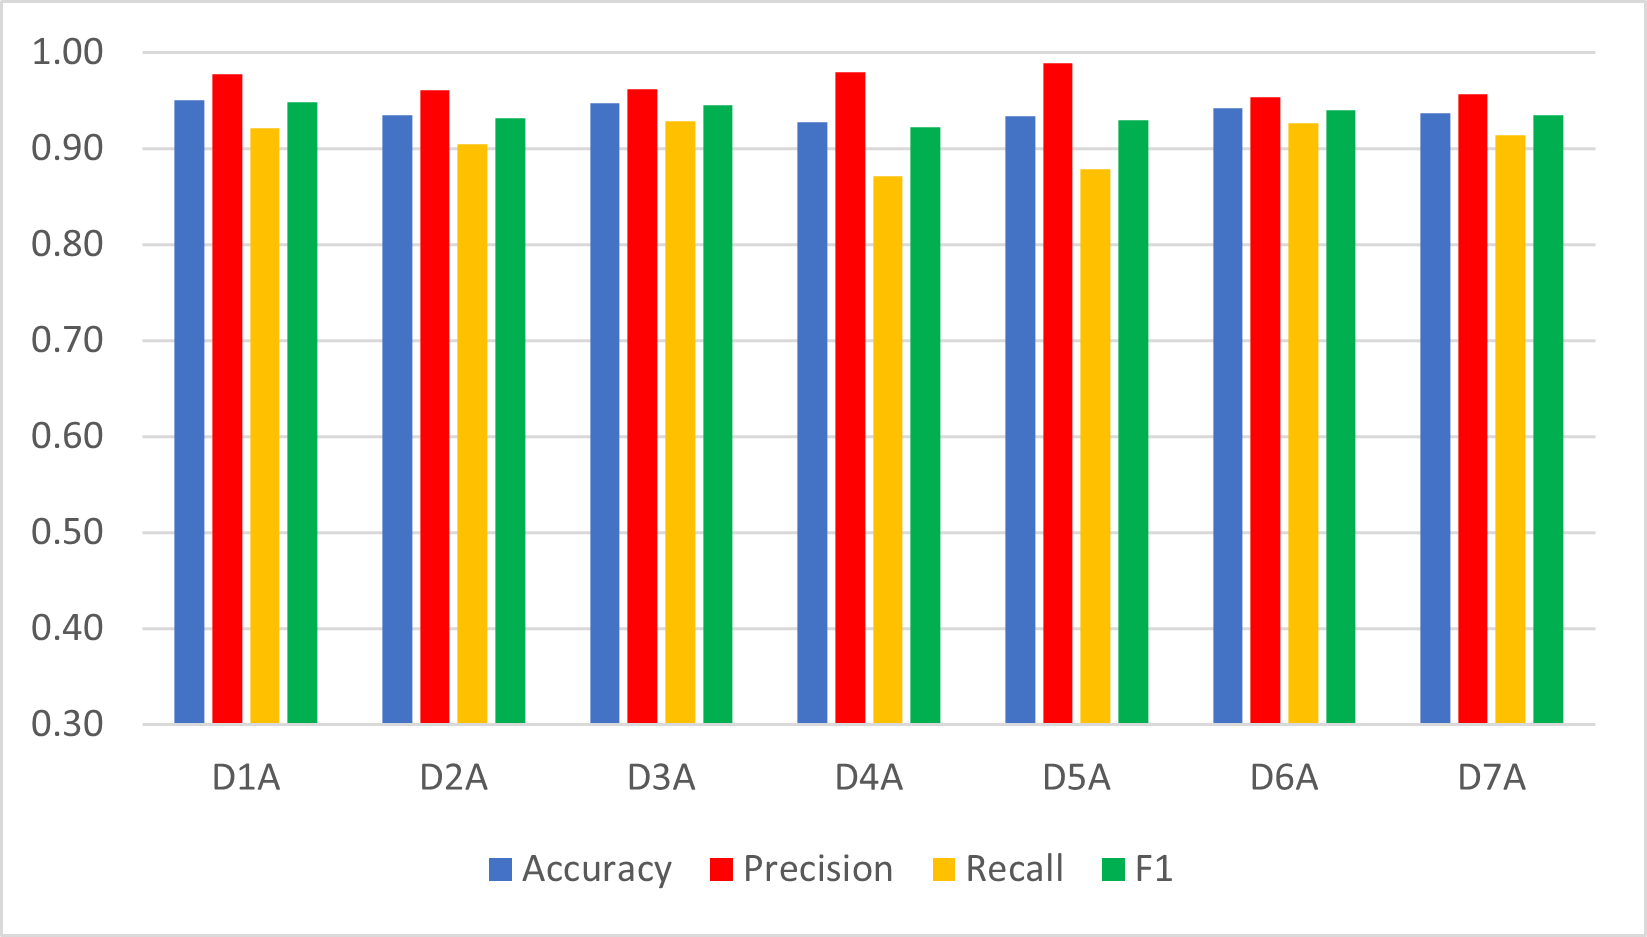
\includegraphics[scale=0.8]{figures/ResultBarGraphs/Anomaly/AC_FreqA.png}
    \caption{Anomaly Coefficient Calculation Graph (Frequency A)}
    \label{fig:ACFA}
\end{figure}

\begin{figure} [H]
    \centering
    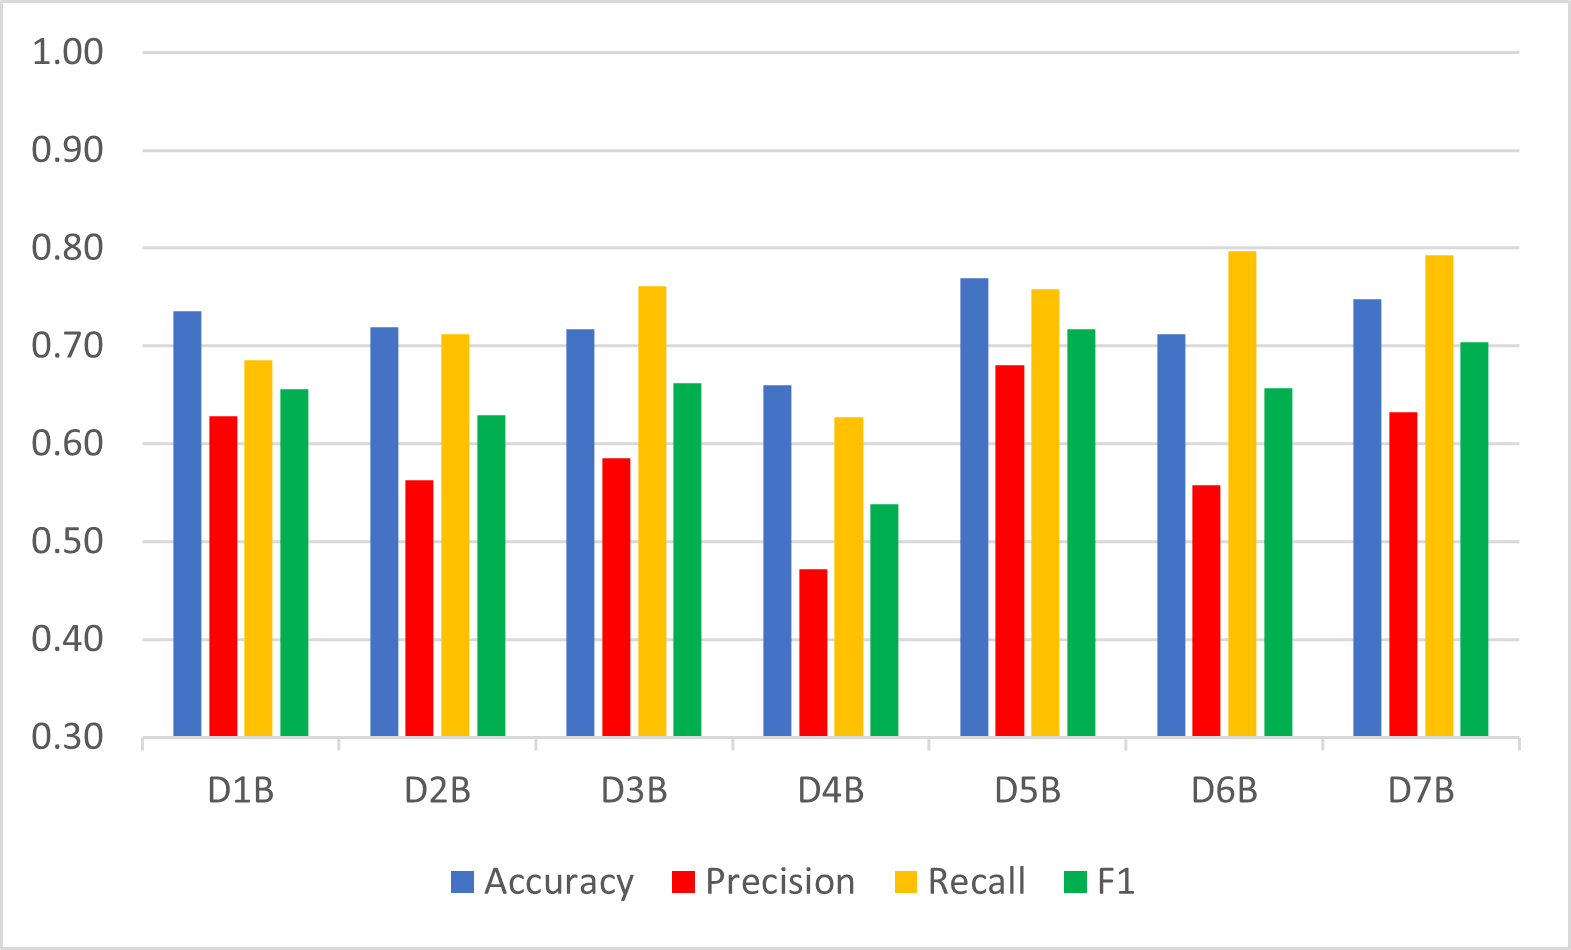
\includegraphics[scale=0.82]{figures/ResultBarGraphs/Anomaly/AC_FreqB.png}
    \caption{Anomaly Coefficient Calculation Graph (Frequency B)}
    \label{fig:ACFB}
\end{figure}

It can be observed that the results from Figure \ref{fig:ACFA} scored the highest, with Figure \ref{fig:ACBF} as the second highest, and Figure \ref{fig:ACFB} as the lowest. From the results, it can be inferred that the metric scores of this method is significantly affected by the ratio of the number of time frames with theft to the number of households. 

Since the datasets have the same number of benign and malicious points, making it symmetric, and False Negative (FN) and False Positive (FP) are valued the same. Therefore, the accuracy would be the best metric to check. Looking at the accuracy, the performance metric data as shown in Table \ref{tab:ACBF} and \ref{tab:ACFA} both show a successful metric as a classifier, both being above 80\%. The algorithm performed well with an average accuracy of 83.08\% for the dataset that contains both frequencies and an average accuracy of 93.88\% for the dataset that contains only frequency A. However, it can be seen in Table \ref{tab:ACFB} that the case with only Frequency B did not have the same success as seen in the other cases. Having only an average of 72.28\%, it fails to achieve an accuracy of at least 80\%.

As seen in the Figures \ref{fig:ACBF}, \ref{fig:ACFA}, and \ref{fig:ACFB}, unlike in SVM and ANN, there is no decreasing trend between the performance metrics of the seven different datasets in each case. This suggests that varying PV and Net Metering penetration do not have a clear effect on Anomaly Coefficient Calculation. The reason behind this is attributed to the fact that the introduction of PV and Net Metering arithmetically adds and subtracts values to both sides of the linear equations (Equation \ref{equation:MatrixInvAC}). The PV generation of a household will be 'deducted' from its meter reading, and the same value will also be subtracted from check meter reading. For houses with Net Metering, the same reason applies, the only difference is that the meter reading of the household may become negative. Therefore, the equation that is used to solve for \(k\) remains unchanged.

The slight differences in the anomaly coefficients \(k\) are attributed to the randomness of the datasets during the simulations, since each of the seven datasets used different load curves and PV generation curves. This also explains the smalls differences in accuracy, precision, recall and F1 scores across the different datasets.

\section{Comparison of Algorithm Results}
\label{section:sec05_02}

Theft detection methods using SVM and ANN detect whether theft is present in the system. On the other hand, Anomaly Coefficient Calculation not only detects theft, but also pinpoints which household is the pilferer. Because of this, the metric scores of SVM and ANN cannot be compared directly to that of the Anomaly Coefficient Calculation.

To identify the cause of the decreasing trend in classifier performance of both ANN and SVM when PV and Net Metering penetration is increased, the characteristics of the datasets were examined. When theft is present, the most obvious fact is that the \% loss error of the check meter that the pilferer belongs to increased significantly.

In order to examine how the percent error values change as PV and NM penetration are varied, the distribution is plotted using histograms. This also illustrates the possible values of the \% loss error of every dataset.

\begin{figure} [H]
    \centering
    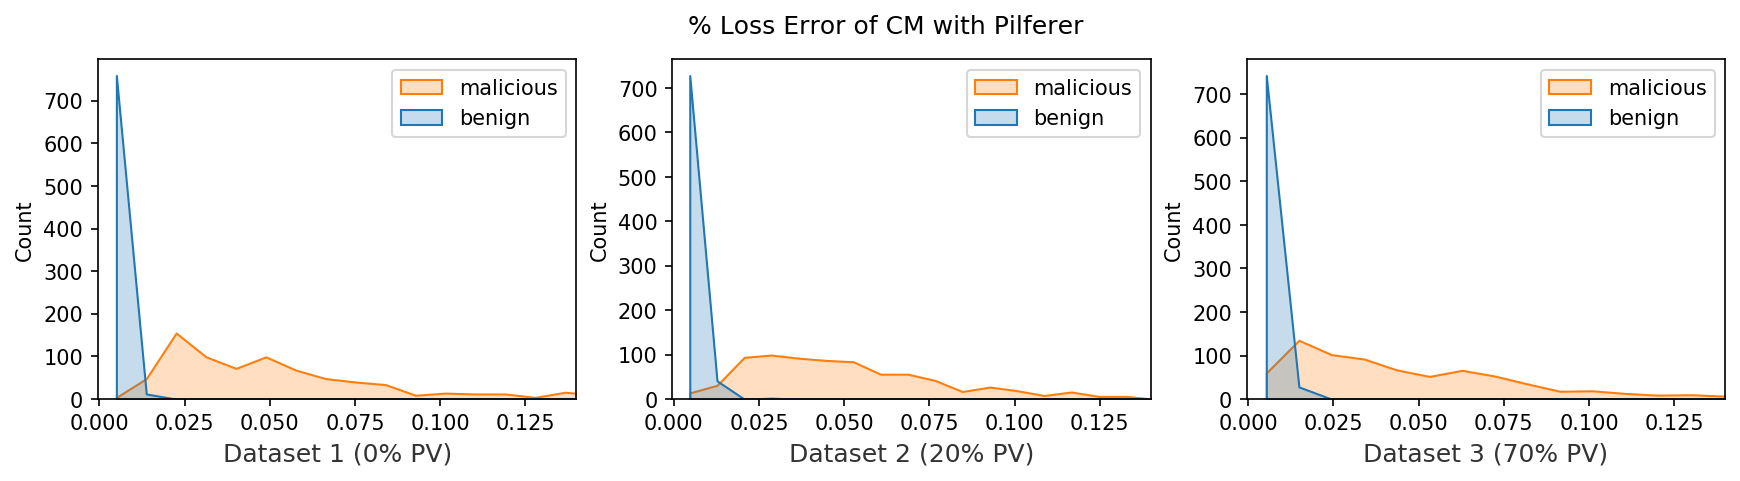
\includegraphics[scale=0.555]{figures/References/histo123.png}
    \caption{Histogram of \% Loss Error for Datasets 1, 2, and 3}
    \label{fig:Histo123}
\end{figure}

Figure \ref{fig:Histo123} shows the histogram plots of the \% Loss Error of the check meter in which the pilferer is present using Datasets 1, 2, and 3. Note that for Datasets 1, 2, and 3, only the PV penetration is varied at 0\%, 20\%, and 70\% penetration respectively. The y-axis represents the number of occurrences while the x-axis represents the \% loss error value. For the three datasets, the benign data points lie mostly on the postive values most near to 0; the slight deviation from 0 is attributed to technical losses caused by the transmission lines. When theft is present, the \% loss error increases and moves further to the right. This is because the pilferer decreases their smart meter readings significantly which causes large deviation from the check meter readings, hence the increase in \% loss error. However, as the PV penetration is increased, the distribution of the \% loss error of the malicious data moves closer to that of the benign data. The distance between the mode of the malicious data and the mode of the benign data decreases which creates an overlap in their distribution. This made it harder for the SVM and ANN classifiers to separate the two classes. Notice that the amount of overlap in Dataset 1 and 2 are almost the same; this is supported by the similar metric scores of Datasets 1 and 2 in both ANN and SVM. In SVM, the accuracy scores of Dataset 1 and 2 are 97\% and 96.5\%, respectively. While in ANN, the accuracy scores are 98\% and 97.3\%, respectively. The small amount of households installed with PV in Dataset 2 has little to no effect in the performance of the classifiers.

\begin{figure} [H]
    \centering
    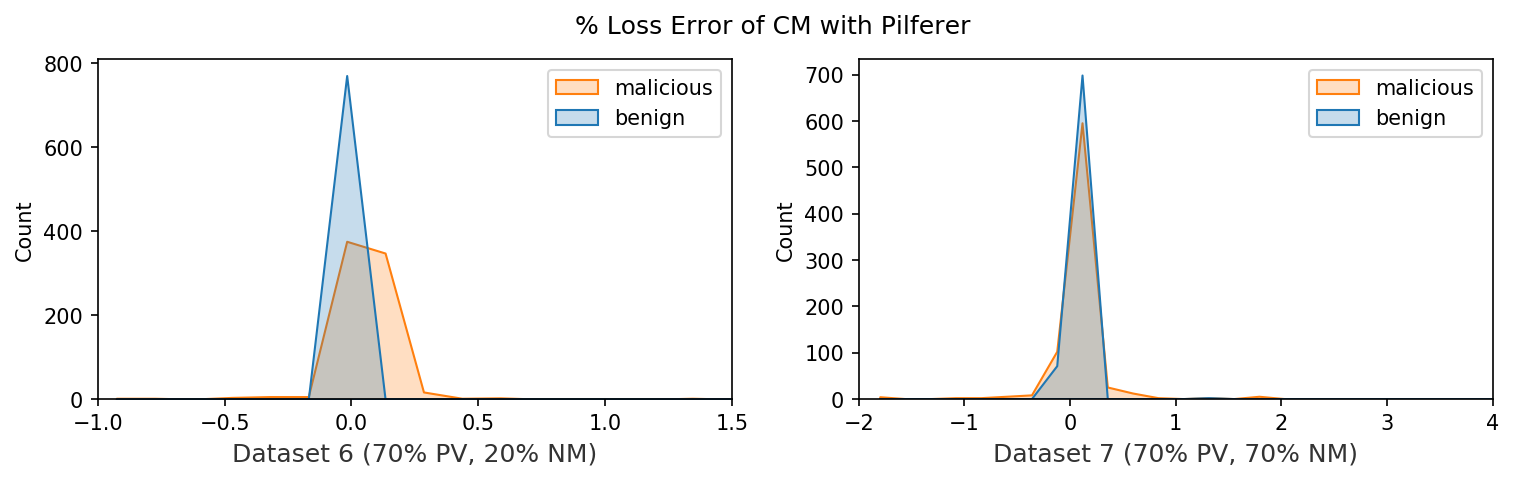
\includegraphics[scale=0.65]{figures/References/histo67.png}
    \caption{Histogram of \% Loss Error for Datasets 6 and 7}
    \label{fig:Histo67}
\end{figure}

To characterize the effect of Net Metering, the histogram plots of Datasets 6 and 7 are compared. Figure \ref{fig:Histo67} shows the histogram plot of Datasets 6 and 7, in which PV penetration is constant at 70\% while Net Metering penetration is at 20\% and 70\%, respectively. To reiterate, the formula for \% loss error of a check meter is given by
\[\% error_i = \frac{\abs{\sum_{n=1}^{k}M_n-CM_i}}{CM_i}\]
where \(CM_i\) is the reading of check meter \emph{i} and \(\sum_{n=1}^{k}M_n\) is the sum of the household meter readings under check meter \emph{i}. The distribution plots shows that there could be negative values of \% loss error for benign data points. This only happens when the net reading of the check meter is negative, which means that the grid receives power from the loads instead of delivering it: the total generated energy exceeds the total consumption of the nearby households. This usually occurs when most of the households under the check meter uses Net Metering.

In Dataset 6, most of distribution curve of the malicious data points overlap that of the benign data points, while in Dataset 7, the malicious data points overlaps the benign data points almost completely. In these two datasets, the classifier's performance is drastically reduced because it cannot separate the two classes anymore; the accuracy scores of Dataset 7 for SVM and ANN are 59.85\% and 63.74\% respectively, the lowest out of all datasets. In a system that has a high PV and NM penetration, the pilferer's activity is harder to detect because the possible range of values for the \% loss error is widened.

High positive values of \% loss error in both the benign and malicious data points happen when the net reading of the check meter is a small positive number, which means that the grid is delivering a very small amount of energy to the households. In this scenario, the total consumption of the nearby households is only slightly greater than the total generated energy of the PVs.

On the other hand, when a pilferer is present, the \% loss error becomes a large negative value. This is the scenario in which the pilferer is a household with an already negative meter reading (production is much larger than consumption). When theft is applied, $k_{et}$ from Section \ref{section:sec04_02_04} is multiplied to an already negative value. This action will translate to a customer increasing their actual rooftop PV generation. This could happen in real life because the main incentive of Net Metering is that excess energy exported to the grid is paid for by the distribution utility company.

Therefore, it is evident that the \% loss error of check meters is not the best feature to use in developing electricity theft classifiers for networks that has a high number of households with PV and Net Metering installed. High penetration values of PV and Net Metering alters the distribution curve of the \% loss error and consequently, the classifier's ability to generalize is worsened hence the decreasing trend of performance metrics. Based on the results, Net Metering penetration affects the performance of the classifiers more than PV penetration alone. This is because of the increased possibility of negative check meter readings which affects the \% loss error calculation.

For networks with low PV penetration, the use of \% loss error as a feature is more than capable in detecting electricity theft. The main advantage of using this kind of feature is its intuitiveness and simplicity; it is easily calculated using check meter and household meter readings which are readily accessible measurements.

%%%%%%%%%%%%%%%%%%%%%%%%%%%%%%%%%%%%%%%%%%%%%%%%%%%%%%%%%%%%%%%%%%%
\chapter{Conclusion and Recommendations\label{cha:chap06}}

This study explored the effect of rooftop PVs and Net Metering on theft detection algorithms. The results showed that the presence of PV and Net Metering in the system significantly affected the performance of SVM and ANN trained on datasets with \% loss error of check meters and household smart meter readings as its features. Due to the nature of how \% loss error is calculated, the presence of PV and Net Metering alters and shifts the distribution of the \% loss error values which makes it harder for the SVM and ANN classifiers to distinguish between benign and malicious data.

With the use of \% loss error as the main feature for datasets trained on SVM and ANN, increasing PV and Net Metering penetration caused a decreasing trend in the metric scores of these algorithms. At low levels of PV penetration, the algorithms performed outstandingly, with accuracy scores as high as 98\% for ANN and 97\% for SVM. However, systems with very high Net Metering penetration performed the worst with accuracy scores as low as 64\% for ANN and 60\% for SVM. Despite its intuitiveness and accessibility, using \% loss error of check meters as one of the dataset features is not the best choice especially in systems with high PV and Net Metering penetration.

For the Anomaly Coefficient Calculation method, results show that the presence of PV and Net Metering does not affect the performance of the algorithm. It was inferred that the small differences in accuracy across the datasets are caused by the randomness of the input load and generation curves. Having lesser time frames or meter readings result in a drastic decrease in accuracy. It is best to use this algorithm when the given data has sufficient data points. 

For future works regarding SVM and ANN, it is recommended to identify better features that can generalize data regardless if PV or Net Metering is present. The performance of these algorithms can also be explored further by introducing systems with different forms of theft. Different theft detection algorithms can be explored that are capable of identifying the pilferer even in cases where the theft frequency is irregular.

\begin{comment}
\begin{equation}
\begin{split}
& x_{m} = \{E_1, E_2, ..., E_8, M_1, M_2, ..., M_{55}, L\} \\
& X=
\begin{bmatrix}
x_{1} && L_1 \\
x_{2} && L_2 \\
x_{3} && L_3 \\
\vdots &&\vdots \\
x_{1540} && L_{1540} \\
\end{bmatrix}
\end{split}
\end{equation}
\end{comment}

\cleardoublepage{}
\printbibliography
\end{document}

%%%%%%%%%%%%%%%%%%%%%%%%%%%%%%%%%%%%%%%%%%%%%%%%%%%%%%%%%%%%%%%%%%%

